\documentclass[11pt,letterpaper]{article}
\usepackage[T1]{fontenc}
\usepackage[utf8]{inputenc}
\usepackage{mathptmx}
\usepackage[margin=1in]{geometry}
\usepackage{amsmath,amssymb}
\usepackage{graphicx}
\usepackage{enumitem}
\usepackage[table]{xcolor}
\usepackage{booktabs,array,longtable}
\usepackage{setspace}
\usepackage{float}
\usepackage{microtype}
\usepackage{titlesec}
\usepackage{fancyhdr}
\usepackage[font=small,labelfont=bf,labelsep=period,justification=raggedright,singlelinecheck=false]{caption}
\captionsetup[figure]{name=Fig.}
\usepackage[hidelinks]{hyperref}
\definecolor{navy}{HTML}{1F3864}
\titleformat{\section}{\large\bfseries\sffamily}{}{0pt}{}
\titleformat{\subsection}{\normalsize\bfseries\itshape}{}{0pt}{}
\titleformat{\subsubsection}{\normalsize\itshape}{}{0pt}{}
\titlespacing*{\section}{0pt}{16pt}{6pt}
\titlespacing*{\subsection}{0pt}{10pt}{3pt}
\titlespacing*{\subsubsection}{0pt}{8pt}{2pt}
\setlength{\parindent}{0pt}\setlength{\parskip}{6pt}
\onehalfspacing
\pagestyle{fancy}\fancyhf{}\renewcommand{\headrulewidth}{0pt}
\fancyfoot[C]{\footnotesize\thepage}
\setlength{\tabcolsep}{5pt}\renewcommand{\arraystretch}{1.12}
\allowdisplaybreaks\emergencystretch=2em
\renewcommand{\floatpagefraction}{0.8}\renewcommand{\textfraction}{0.1}

\newcommand{\NExtract}{3,476,180}
\newcommand{\NResident}{3,467,679}
\newcommand{\NTotal}{3,259,496}
\newcommand{\PctKept}{93.77}
\newcommand{\NExcluded}{208,183}
\newcommand{\NSmokers}{97,187}
\newcommand{\PrevSmoke}{2.98}
\newcommand{\PretermAll}{8.47}
\newcommand{\PretermSmk}{13.9}
\newcommand{\PretermNon}{8.3}
\newcommand{\PretermSmkTwo}{13.90}
\newcommand{\PretermNonTwo}{8.30}
\newcommand{\GAsmk}{37.97}
\newcommand{\GAnon}{38.45}
\newcommand{\DroppedPreterm}{12.1}
\newcommand{\KeptPreterm}{8.5}
\newcommand{\DroppedSmoke}{3.13}
\newcommand{\KeptSmoke}{2.98}
\newcommand{\NDropped}{208,183}
\newcommand{\CrudeRD}{5.60}
\newcommand{\CrudeLo}{5.38}
\newcommand{\CrudeHi}{5.82}
\newcommand{\RDmain}{3.26}
\newcommand{\RDlo}{2.47}
\newcommand{\RDhi}{4.04}
\newcommand{\SEmain}{0.399}
\newcommand{\RRmain}{1.39}
\newcommand{\RRcrude}{1.68}
\newcommand{\RDg}{3.48}
\newcommand{\RDiptw}{3.53}
\newcommand{\RDiptwLo}{2.77}
\newcommand{\RDiptwHi}{4.30}
\newcommand{\ATT}{3.39}
\newcommand{\ATTlo}{3.17}
\newcommand{\ATThi}{3.61}
\newcommand{\ATO}{3.30}
\newcommand{\ATOlo}{3.08}
\newcommand{\ATOhi}{3.52}
\newcommand{\ReducePct}{42}
\newcommand{\PerK}{34}
\newcommand{\RRlo}{1.30}
\newcommand{\EV}{2.12}
\newcommand{\EVlo}{1.92}
\newcommand{\RRhi}{1.48}
\newcommand{\RDPre}{3.65}
\newcommand{\RDPreLo}{2.88}
\newcommand{\RDPreHi}{4.43}
\newcommand{\RDIns}{3.05}
\newcommand{\RDInsLo}{2.23}
\newcommand{\RDInsHi}{3.87}
\newcommand{\RDInt}{3.02}
\newcommand{\RDIntLo}{2.46}
\newcommand{\RDIntHi}{3.59}
\newcommand{\RDFive}{3.22}
\newcommand{\RDFiveLo}{2.72}
\newcommand{\RDFiveHi}{3.72}
\newcommand{\RangeMin}{3.02}
\newcommand{\RangeMax}{3.65}
\newcommand{\PreShift}{0.40}
\newcommand{\RDnoclamp}{3.38}
\newcommand{\RDtrim}{3.03}
\newcommand{\TrimKeep}{60.3}
\newcommand{\MaxWtClamp}{187}
\newcommand{\MaxWtNone}{453}
\newcommand{\ESSclamp}{6,806}
\newcommand{\ESSnone}{5,134}
\newcommand{\NLevels}{38}
\newcommand{\BalBefore}{21}
\newcommand{\BalAfter}{3}
\newcommand{\BalOv}{0}
\newcommand{\SMDbefore}{0.64}
\newcommand{\SMDafter}{0.13}
\newcommand{\SMDov}{0.00}
\newcommand{\LowNon}{41}
\newcommand{\LowSmk}{4.1}
\newcommand{\LowBach}{56}
\newcommand{\LowMast}{27}
\newcommand{\LowDoc}{8}
\newcommand{\LowBachSum}{91}
\newcommand{\SEif}{0.399}
\newcommand{\SEboot}{0.388}
\newcommand{\SEratio}{0.97}
\newcommand{\BootLo}{2.55}
\newcommand{\BootHi}{4.08}
\newcommand{\BootB}{1,000}
\newcommand{\BootMean}{3.25}
\newcommand{\CFLog}{3.22}
\newcommand{\CFLogLo}{2.43}
\newcommand{\CFLogHi}{4.01}
\newcommand{\CFwLog}{3.52}
\newcommand{\CFoLog}{3.48}
\newcommand{\CFLasso}{2.80}
\newcommand{\CFLassoLo}{2.02}
\newcommand{\CFLassoHi}{3.57}
\newcommand{\CFwLasso}{3.01}
\newcommand{\CFoLasso}{3.85}
\newcommand{\CFForest}{2.30}
\newcommand{\CFForestLo}{1.39}
\newcommand{\CFForestHi}{3.21}
\newcommand{\CFwForest}{2.51}
\newcommand{\CFoForest}{3.77}
\newcommand{\CFAvg}{2.84}
\newcommand{\CFAvgLo}{2.28}
\newcommand{\CFAvgHi}{3.41}
\newcommand{\CFwAvg}{3.00}
\newcommand{\CFoAvg}{3.70}
\newcommand{\CFreps}{2}
\newcommand{\CFrange}{0.08}
\newcommand{\ContQuit}{3.08}
\newcommand{\ContQuitLo}{2.56}
\newcommand{\ContQuitHi}{3.59}
\newcommand{\ContQuitPre}{3.63}
\newcommand{\QuitNever}{-0.07}
\newcommand{\QuitNeverLo}{-0.40}
\newcommand{\QuitNeverHi}{0.27}
\newcommand{\QuitNeverATE}{0.53}
\newcommand{\HistNever}{8.3}
\newcommand{\HistQuit}{9.4}
\newcommand{\HistCont}{13.9}
\newcommand{\HistStart}{12.5}
\newcommand{\NQuit}{27,794}
\newcommand{\NCont}{94,650}
\newcommand{\NStart}{2,395}
\newcommand{\NNever}{3,134,250}
\newcommand{\DoseMin}{3.27}
\newcommand{\DoseMax}{3.55}
\newcommand{\EducShare}{46}
\newcommand{\PPShare}{38}
\newcommand{\EducChange}{1.03}
\newcommand{\PPChange}{0.33}
\newcommand{\PrecareChange}{0.64}
\newcommand{\WicChange}{-0.13}
\newcommand{\PrecareShareOut}{11}
\newcommand{\ExcessPerK}{34}
\newcommand{\ExcessBirths}{3,300}
\newcommand{\OneIn}{30}
\newcommand{\ExcessBirthsExact}{3,293}
\newcommand{\ExcessLo}{3,100}
\newcommand{\ExcessHi}{3,500}
\newcommand{\PPsmk}{8.9}
\newcommand{\PPnon}{3.7}
\newcommand{\PPrisk}{26.1}
\newcommand{\NoPPrisk}{7.6}
\newcommand{\SmkNoDip}{8.4}
\newcommand{\SmkDoc}{0.1}
\newcommand{\VeducSmk}{0.15}
\newcommand{\VppPre}{0.13}
\newcommand{\VeducWic}{0.42}
\newcommand{\TriN}{3,218,258}
\newcommand{\TriNever}{7.94}
\newcommand{\TriFirst}{10.73}
\newcommand{\TriFirstSecond}{13.18}
\newcommand{\TriAll}{13.93}
\newcommand{\TriLate}{10.75}
\newcommand{\TriLateN}{2,288}
\newcommand{\TriAATT}{1.38}
\newcommand{\TriALo}{0.86}
\newcommand{\TriAHi}{1.90}
\newcommand{\TriBATT}{3.43}
\newcommand{\TriBLo}{2.55}
\newcommand{\TriBHi}{4.31}
\newcommand{\TriCATT}{3.68}
\newcommand{\TriCLo}{3.43}
\newcommand{\TriCHi}{3.93}
\newcommand{\TriDATT}{0.87}
\newcommand{\TriDLo}{$-$0.36}
\newcommand{\TriDHi}{2.11}
\newcommand{\TriDoseA}{3.26}
\newcommand{\TriDoseLoA}{2.89}
\newcommand{\TriDoseHiA}{3.63}
\newcommand{\TriDoseB}{3.72}
\newcommand{\TriDoseLoB}{3.32}
\newcommand{\TriDoseHiB}{4.12}
\newcommand{\TriDoseC}{4.44}
\newcommand{\TriDoseLoC}{3.85}
\newcommand{\TriDoseHiC}{5.03}
\newcommand{\TriDoseD}{5.03}
\newcommand{\TriDoseLoD}{3.26}
\newcommand{\TriDoseHiD}{6.80}
\newcommand{\TriDoseWideATE}{11.02}
\newcommand{\TriDoseWideLo}{$-$2.17}
\newcommand{\TriDoseWideHi}{24.20}

\graphicspath{{figs/}}
\hypersetup{pdftitle={Smoking during pregnancy and preterm birth: a doubly robust analysis of 3.26 million U.S. births},pdfauthor={Faruk Muritala and Dhrubajyoti Ghosh}}
\begin{document}

\begin{flushleft}
{\LARGE\bfseries Smoking during pregnancy and preterm birth: a doubly robust propensity score weighting analysis of 3.26 million U.S. births}\\[14pt]
{\large Faruk Muritala$^{1*}$ and Dhrubajyoti Ghosh$^{1}$}\\[8pt]
$^{1}$Department of Data Science and Analytics, Kennesaw State University, Georgia, USA\\[2pt]
$^{*}$Corresponding author\\[10pt]
\textit{Manuscript prepared for submission to BMC Pregnancy and Childbirth.}
\end{flushleft}

\section*{Abstract}
\textbf{Background.} Smoking during pregnancy is a modifiable risk factor for preterm birth. Large U.S. analyses report adjusted odds ratios from a single regression model, which gives no absolute risk and does not show how much of the estimate rests on mothers who have comparable counterparts. This study estimated the effect of smoking on preterm birth as a risk difference and examined each assumption behind it.

\textbf{Methods.} Singleton live births from the 2023 U.S. Natality Public Use File were analysed (\NTotal{} births with complete data, \NSmokers{} to mothers who smoked). The exposure was any cigarette smoking during pregnancy and the outcome was birth before 37 completed weeks. Ten confounders were chosen from a causal diagram. The risk difference was estimated by augmented inverse probability of treatment weighting (AIPTW), which gives a valid estimate if either the smoking model or the outcome model is correct. Overlap and covariate balance were examined, the standard error was checked against a full-sample bootstrap, LASSO and random forest models were fitted with five-fold cross-fitting, and an E-value was computed.

\textbf{Results.} The crude difference in preterm birth was \CrudeRD{} percentage points. After adjustment it was \RDmain{} points (bootstrap 95\% CI \BootLo{} to \BootHi{}; risk ratio \RRmain{}), and \ATT{} points among mothers who smoked (\ATTlo{} to \ATThi{}), about \ExcessPerK{} additional preterm births per 1,000 smoking pregnancies. The bootstrap standard error was \SEboot{} against \SEif{} from the influence function. Estimates ranged from \RangeMin{} to \RangeMax{} across covariate sets and propensity score rules, and from \CFForest{} to \CFLasso{} with cross-fitted random forest and LASSO models. Overlap was limited: \LowNon{}\% of non-smokers had an estimated probability of smoking below 0.01. The E-value was \EV{}. In exploratory analyses, the effect among smokers was \TriAATT{} points for smoking in the first trimester only and \TriCATT{} points for smoking in all three trimesters, and mothers who quit before pregnancy resembled mothers who never smoked.

\textbf{Conclusions.} Under the stated assumptions, smoking during pregnancy raised the absolute risk of preterm birth by about three percentage points, a result that held across flexible models, a full bootstrap and changes in the adjustment set. It rests on self-reported smoking, limited overlap and the assumption of no unmeasured confounding.

\textbf{Keywords:} preterm birth, maternal smoking, causal inference, doubly robust estimation, cross-fitting, propensity score, E-value

\section*{Background}

Preterm birth, delivery before 37 completed weeks of gestation, affected 10.41\% of U.S. births in 2023 \cite{martin2024}. Cigarette smoking during pregnancy is one of the few causes that can be changed. The share of U.S. mothers who smoked during pregnancy fell from 7.2\% in 2016 to 4.6\% in 2021, and the decline left large differences between groups, with the highest rates among non-Hispanic American Indian or Alaska Native (12.7\%) and non-Hispanic White (6.7\%) mothers \cite{martin2023}.

The strongest recent evidence on smoking and preterm birth comes from birth certificates. A study of 25,623,479 U.S. singleton births from 2011 to 2018 reported adjusted odds ratios for preterm birth that rose with cigarettes smoked per day, from 1.31 for one to two cigarettes to 1.53 for twenty or more in the first trimester, and found risk comparable to non-smokers among women who quit before pregnancy \cite{liu2020}. A commentary noted that studies of this question disagree, that cessation subgroups are small, and that results depend on how pre-pregnancy quitters are classified and when smoking is measured \cite{stock2020}. Other natality-file analyses use regression to estimate odds ratios and, in one case, report E-values for unmeasured confounding \cite{kondracki2020}.

Three limits follow from this work. Odds ratios from one logistic regression depend on that model being correct, and they do not give the absolute change in risk used to plan services. Regression does not show whether smokers and non-smokers overlap on the measured characteristics, so a reader cannot tell how much of an estimate rests on comparable mothers and how much on extrapolation. The adjustment set is rarely tied to a causal diagram that separates characteristics fixed before pregnancy from those recorded during it.

This study addresses these limits with the 2023 U.S. natality file. Ten confounders were chosen from a causal diagram. The effect of smoking on preterm birth was estimated as an absolute risk difference with AIPTW, which remains consistent if either the propensity model or the outcome model is correct \cite{bang2005}. The identifying assumptions are stated and each one is examined. Overlap was assessed through the propensity score distribution, the effective sample size and covariate balance. The standard error was checked against a full-sample bootstrap, the nuisance models were fitted flexibly with cross-fitting \cite{chern2018}, and the estimate was repeated under alternative propensity score rules and covariate sets. The E-value quantifies the strength of an unmeasured confounder needed to explain the estimate away \cite{vdw2017}. Smoking before pregnancy and by trimester was then used to compare mothers who continued to smoke with mothers who stopped.

\section*{Methods}

\subsection*{Data source and study population}
The 2023 Natality Public Use File of the National Center for Health Statistics contains a record for every U.S. birth \cite{nchs2024}. A 24-variable extract of \NExtract{} singleton live births with known gestational age and smoking status was used for the main analysis. After excluding births to mothers who were not U.S. residents (\NResident{} remaining) and births with a missing value for any confounder, \NTotal{} births (\PctKept{}\% of the extract) formed the analytic cohort. Births in the cohort were less likely to be preterm than the \NDropped{} births excluded for missing data (\KeptPreterm{}\% against \DroppedPreterm{}\%; Additional file 1, Table S2). The timing of smoking by trimester is recorded only in the full national file, which was used for that analysis alone (see Smoking history and trimester of smoking).

\subsection*{Exposure and outcome}
The exposure was any cigarette smoking during pregnancy, self-reported on the birth certificate. The outcome was preterm birth, a gestational age under 37 completed weeks by the obstetric estimate \cite{martin2015}.

\subsection*{Confounders}
Ten confounders were selected from the causal diagram in Fig.~\ref{fig:dag}: maternal age, race and Hispanic origin, education, timing of prenatal care, participation in the Special Supplemental Nutrition Program for Women, Infants, and Children (WIC), parity, previous preterm birth, pre-pregnancy diabetes, pre-pregnancy hypertension and pre-pregnancy body mass index. Age and body mass index entered as categories, so no straight-line relationship was assumed. Additional file 1 (Table S1) lists every variable, its levels and its share of missing values. The diagram follows published guidance on confounder selection \cite{tennant2021,pearl1995}. Prenatal-care timing and WIC are recorded during pregnancy and may be influenced by smoking or by the length of the pregnancy itself \cite{shin2019,joyce2008,heaman2008}, so every analysis was repeated without them.

\begin{figure}[htbp]
\centering
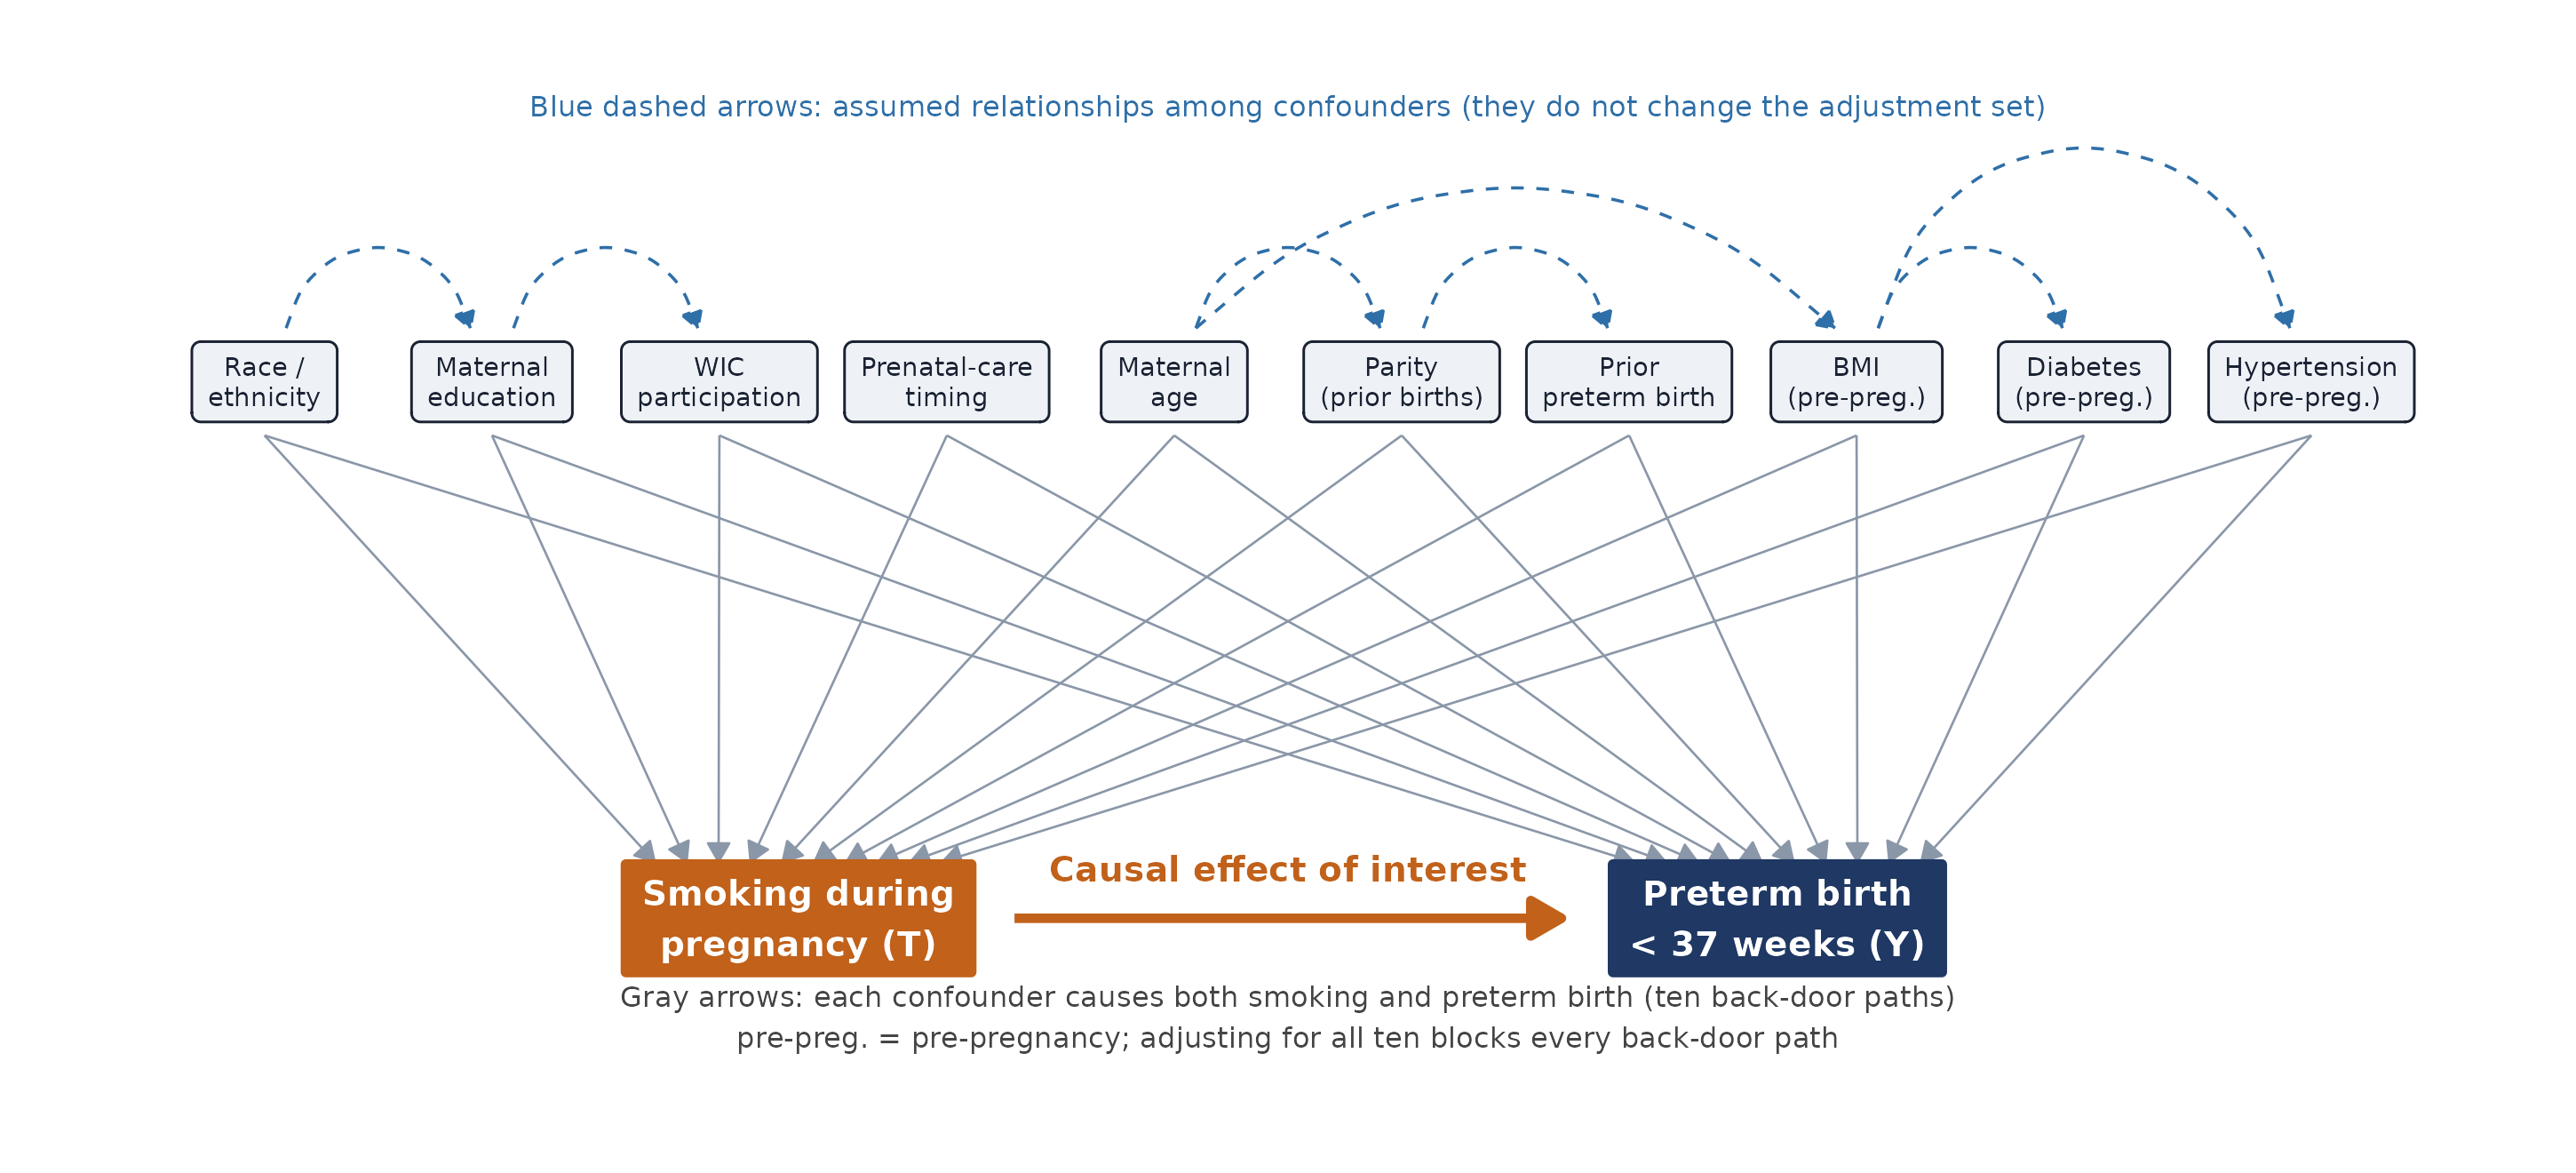
\includegraphics[width=\textwidth]{fig_dag.png}
\caption{Causal diagram. The exposure is smoking in pregnancy ($T$, orange) and the outcome is preterm birth ($Y$, navy). Each confounder is a parent of both. Dashed blue arrows are assumed relationships among confounders. Dashed boxes mark variables measured during pregnancy.}\label{fig:dag}
\end{figure}

\subsection*{Causal estimand and identifying assumptions}
Let $T$ indicate smoking during pregnancy, $Y$ indicate preterm birth, $X$ be the ten confounders, and $Y(1)$ and $Y(0)$ be the potential outcomes of a mother if she smoked or did not smoke \cite{rubin1974}. The average treatment effect (ATE) is $\mathrm{ATE}=\mathbb{E}[Y(1)]-\mathbb{E}[Y(0)]$, the difference in preterm risk if every mother smoked against if none did. The average effect among mothers who smoked (ATT), $\mathbb{E}[Y(1)-Y(0)\mid T=1]$, answers the question for the group that was exposed. A causal reading of either quantity requires the assumptions in Table~\ref{tab:assump}; the first three are the standard conditions for identification \cite{rosenbaum1983,hernan2020}, and the fourth is what makes the estimator doubly robust.

\begin{table}[htbp]
\centering
\caption{Assumptions behind the causal interpretation and how each was examined}\label{tab:assump}
\small
\begin{tabular}{>{\raggedright\arraybackslash}p{3.0cm}>{\raggedright\arraybackslash}p{6.4cm}>{\raggedright\arraybackslash}p{5.6cm}}
\toprule
Assumption & Meaning in this study & How it was examined \\
\midrule
Consistency and no interference & A mother's observed outcome equals her potential outcome under the smoking status she had, and one mother's smoking does not change another mother's outcome. \textquotedblleft Any smoking\textquotedblright{} is treated as one exposure, although dose and timing differ \cite{cole2009}. & Stated. The averaging over dose and timing is relaxed in the smoking history and trimester analyses. \\[4pt]
Conditional exchangeability & Given the ten confounders, mothers who smoked and mothers who did not would have had the same risk of preterm birth under either smoking status. No unmeasured confounder remains. & Cannot be tested. Confounders were chosen from a causal diagram, and the E-value and benchmark covariates give the strength of an unmeasured confounder that would overturn the result. \\[4pt]
Positivity & Every combination of confounder values occurs among both smokers and non-smokers, so $0<e(X)<1$. The ATT needs only that every smoker has non-smoking counterparts. & Propensity score distribution, share of scores below 0.01, largest weights and effective sample size, clamping, overlap weights, and the ATT \cite{petersen2012}. \\[4pt]
Correct model for at least one nuisance function & Either the model for smoking, $e(X)$, or the models for preterm birth, $\mu_t(X)$, describe the data correctly. Both need not be right. & Logistic models, LASSO with interactions and random forests, each cross-fitted, and calibration of predicted against observed risk. \\[4pt]
Accurate measurement and live births & Smoking and gestational age are recorded correctly, or errors are unrelated to the other variables. Only live births are observed. & Discussed under limitations. \\
\bottomrule
\end{tabular}
\end{table}

\subsection*{Statistical analysis}
Let $e(X)=P(T=1\mid X)$ be the propensity score and $\mu_t(X)=P(Y=1\mid T=t,X)$ the chance of preterm birth under smoking status $t$. The AIPTW estimator is
\begin{equation}
\hat\psi_t=\frac1n\sum_{i=1}^{n}\left[\hat\mu_t(X_i)+\frac{\mathbb{1}(T_i=t)\,\big(Y_i-\hat\mu_t(X_i)\big)}{\hat P(T_i=t\mid X_i)}\right],\qquad \widehat{\mathrm{ATE}}=\hat\psi_1-\hat\psi_0 .
\end{equation}
The first term in brackets is the prediction of the outcome model. The second term corrects that prediction by the weighted difference between observed and predicted outcomes, so the estimate is valid if either the outcome model or the propensity model is correct \cite{bang2005,funk2011}. The main analysis used logistic regression with main effects of the ten confounders for $e(X)$, $\mu_1(X)$ and $\mu_0(X)$, and clamped $\hat e$ at its 1st and 99th percentiles. Outcome regression, stabilized inverse probability weighting and overlap weights \cite{li2018} were estimated alongside for comparison. Because births with identical confounder values carry identical predictions, the data were collapsed to 65,787 covariate cells for computation; the results are the same as those from the individual records.

\subsection*{Cross-fitting and flexible nuisance models}
The three functions $e(X)$, $\mu_1(X)$ and $\mu_0(X)$ are called nuisance functions because they are needed to compute the effect but are not the quantity of interest. To check that the result does not depend on the logistic form, they were also estimated by two flexible learners: a logistic regression with all two-way interactions among the confounders, shrunk by the LASSO penalty (penalty chosen by 3-fold cross-validation), and a probability random forest (100 trees). Flexible learners can fit noise in the births they are trained on, so a birth would be given a prediction that is too close to its own outcome. Putting such predictions into the AIPTW formula biases the estimate and makes its standard error too small. Cross-fitting avoids this by never scoring a birth with a model that was trained on it \cite{chern2018,zivich2021}. It was carried out as follows (Fig.~\ref{fig:cf}).

\begin{enumerate}\setlength{\itemsep}{2pt}
\item Each birth was assigned at random to one of five folds of about equal size.
\item For fold $k$, the three nuisance models were fitted on the other four folds only. The propensity model used all births in the four folds, with smoking as the outcome and the ten confounders as predictors. The model $\mu_1$ used only the mothers who smoked in those folds, with preterm birth as the outcome, and $\mu_0$ used only the mothers who did not smoke.
\item The fitted models were used to predict, for every birth in fold $k$, the chance of smoking $\hat e(X)$ and the chance of preterm birth with smoking $\hat\mu_1(X)$ and without smoking $\hat\mu_0(X)$, from that birth's confounders. The outcome of a birth in fold $k$ played no part in producing its own predictions.
\item Steps 2 and 3 were repeated for each of the five folds. The five sets of held-out predictions were then stacked, so that every birth had one value of each function.
\item The AIPTW estimate was computed once from the stacked predictions, with clamping at the 1st and 99th percentiles.
\item The whole procedure was repeated with a second random split of the births, and the two estimates were averaged.
\end{enumerate}

The purpose is twofold. It lets the learners find curved and interacting patterns without being told where to look, and it keeps the standard error honest because the predictions for each birth are made out of sample. To limit memory use, the forest for the propensity score was trained on all smokers and a 10\% random sample of non-smokers in the training folds, with the predicted odds corrected by the sampling fraction, and the forest for non-smokers' outcomes used a 25\% sample. Calibration of predicted against observed risk was checked for each learner.

\begin{figure}[htbp]
\centering
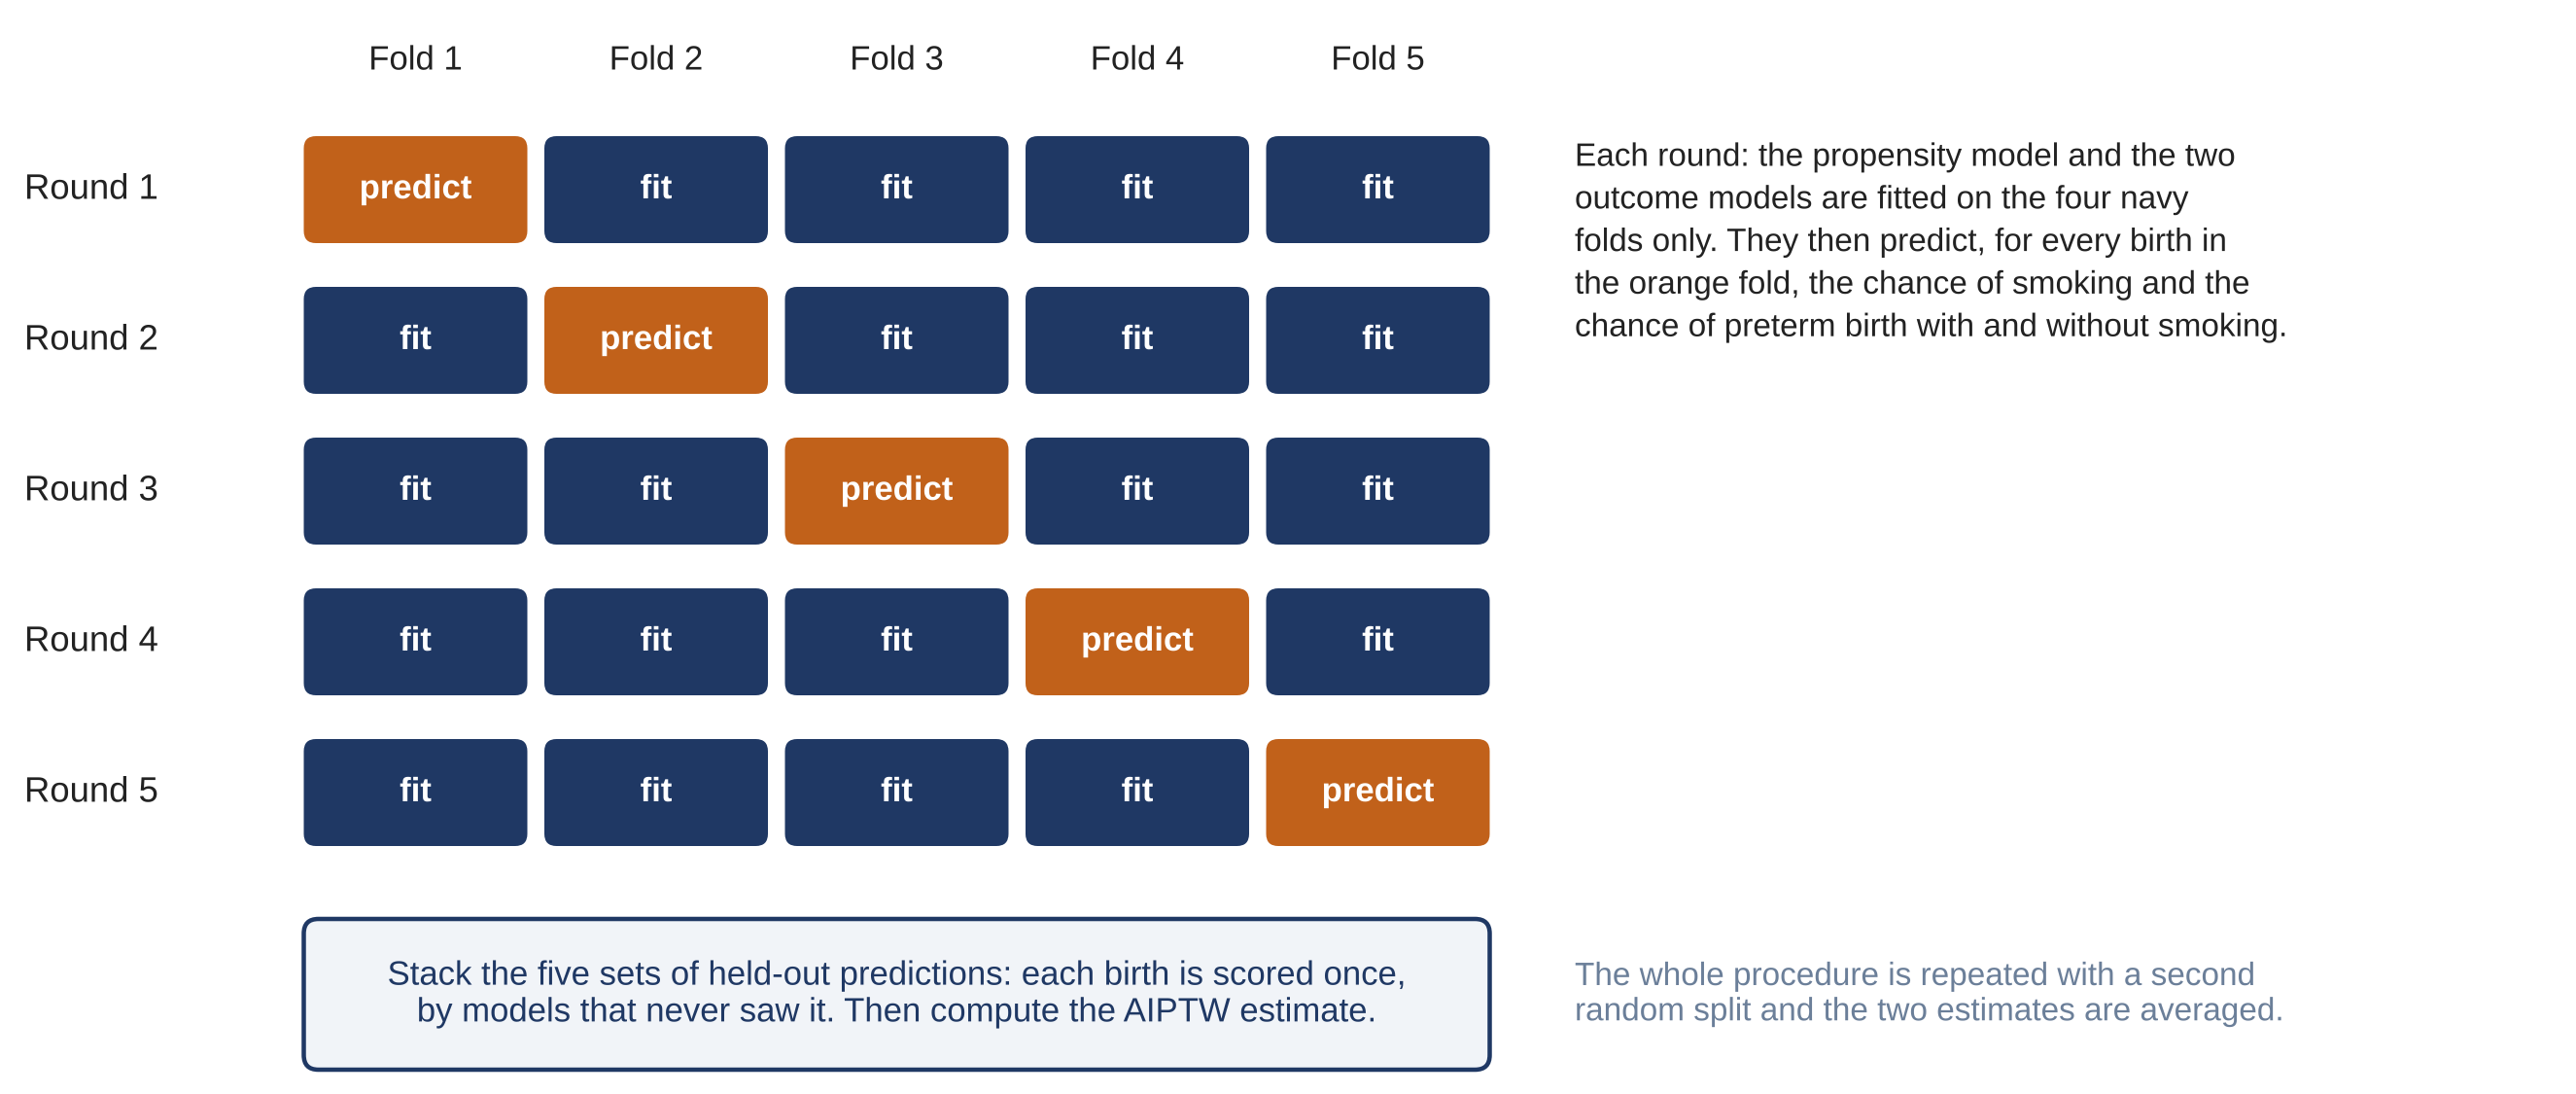
\includegraphics[width=\textwidth]{crossfit_scheme.png}
\caption{Five-fold cross-fitting. In each round, the propensity model and the two outcome models are fitted on the four folds marked ``fit'' and predict for the fold marked ``predict''. The five sets of held-out predictions are stacked before the AIPTW estimate is computed. The procedure is repeated with a second random split.}\label{fig:cf}
\end{figure}

\subsection*{Variance}
The standard error was the empirical standard deviation of the estimated influence function divided by $\sqrt n$. It was compared with a full-sample bootstrap in which the propensity model, both outcome models and the estimator were refitted on each of \BootB{} resamples. Resampling the cell counts from a multinomial distribution is equivalent to resampling births, which made the full-sample bootstrap feasible. The bootstrap percentile interval was taken as the primary interval.

\subsection*{Overlap and balance}
Standardized mean differences (SMD) were computed for every covariate level before and after weighting, and $|{\rm SMD}|>0.10$ was treated as imbalance \cite{austin2015}.

\subsection*{Sensitivity analyses}
The risk difference was re-estimated without clamping, with clamping at the 0.1/99.9 and 5/95 percentiles, after deleting births with scores outside 0.01 to 0.99, without prenatal-care timing and WIC, with insurance type added, and with two-way interactions. The E-value for a risk ratio $\mathrm{RR}$ is $\mathrm{RR}+\sqrt{\mathrm{RR}(\mathrm{RR}-1)}$ \cite{vdw2017}, and measured confounders were used as benchmarks.

\subsection*{Smoking history and trimester of smoking}
The extract records cigarettes per day before pregnancy. Mothers who smoked before but not during pregnancy (``quit'') were compared with those who continued and with those who never smoked. Among those who continued, the effect was estimated by pre-pregnancy intensity. Timing of smoking was studied in the full natality file, where the cohort was rebuilt with the same rules and the effect among those who smoked was estimated for four trimester patterns (first trimester only, first and second trimesters only, all three trimesters, and starting after the first trimester), each against mothers who never smoked, and by third-trimester cigarettes per day among mothers who smoked throughout. These analyses were planned after the main analysis was fixed and are exploratory.

\subsection*{Software}
All analyses used R with a fixed random seed (1234). A single script produces every number, table and figure in this paper.

\section*{Results}

\subsection*{Study population and crude comparison}
Of \NTotal{} births, \NSmokers{} (\PrevSmoke{}\%) were to mothers who reported smoking during pregnancy. Preterm birth occurred in \PretermSmk{}\% of mothers who smoked and \PretermNon{}\% of those who did not, a crude risk difference of \CrudeRD{} points (\CrudeLo{} to \CrudeHi{}). The mean gestational age at delivery was \GAsmk{} weeks for smokers and \GAnon{} weeks for non-smokers. Smoking was concentrated in specific groups (Fig.~\ref{fig:who}): \SmkNoDip{}\% of mothers with 9 to 12 years of schooling and no diploma smoked, against \SmkDoc{}\% of those with a doctorate.

\begin{figure}[htbp]
\centering
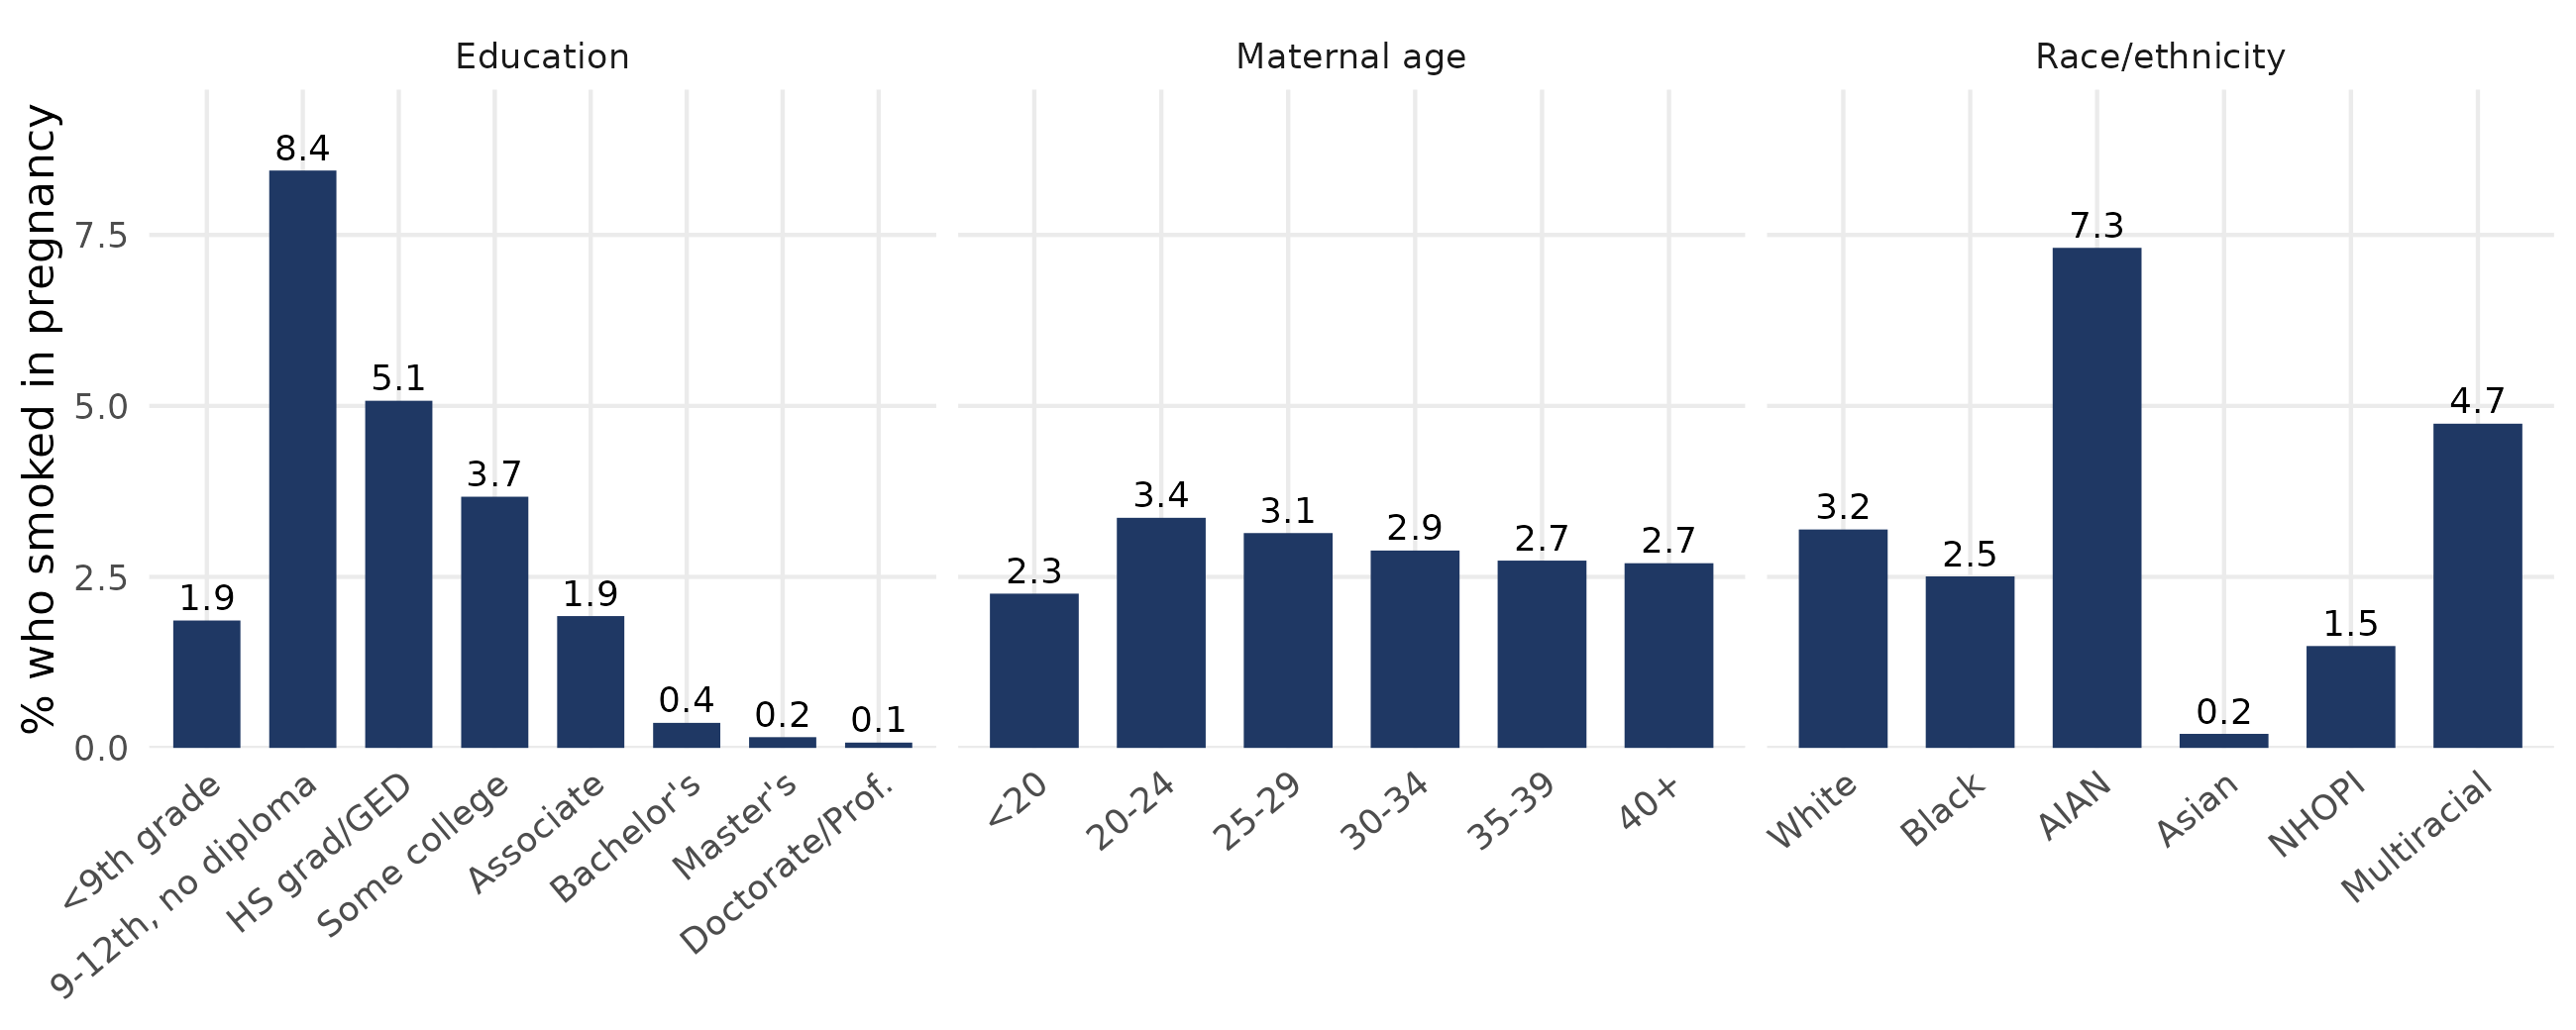
\includegraphics[width=\textwidth]{fig_eda_who_smokes.png}
\caption{Percentage of mothers who smoked during pregnancy by education, age and race and ethnicity.}\label{fig:who}
\end{figure}

\subsection*{Who is compared}
Education was the variable most strongly associated with smoking (Cram\'er's $V$ \VeducSmk{}) and was closely tied to WIC participation ($V=\VeducWic{}$) (Fig.~\ref{fig:corr}). Education accounted for \EducShare{}\% of the fit of the smoking model and a previous preterm birth for \PPShare{}\% of the fit of the preterm-birth model; leaving education out would move the estimate by +\EducChange{} points and leaving out previous preterm birth by +\PPChange{} points (Fig.~\ref{fig:rank}).

\begin{figure}[htbp]
\centering
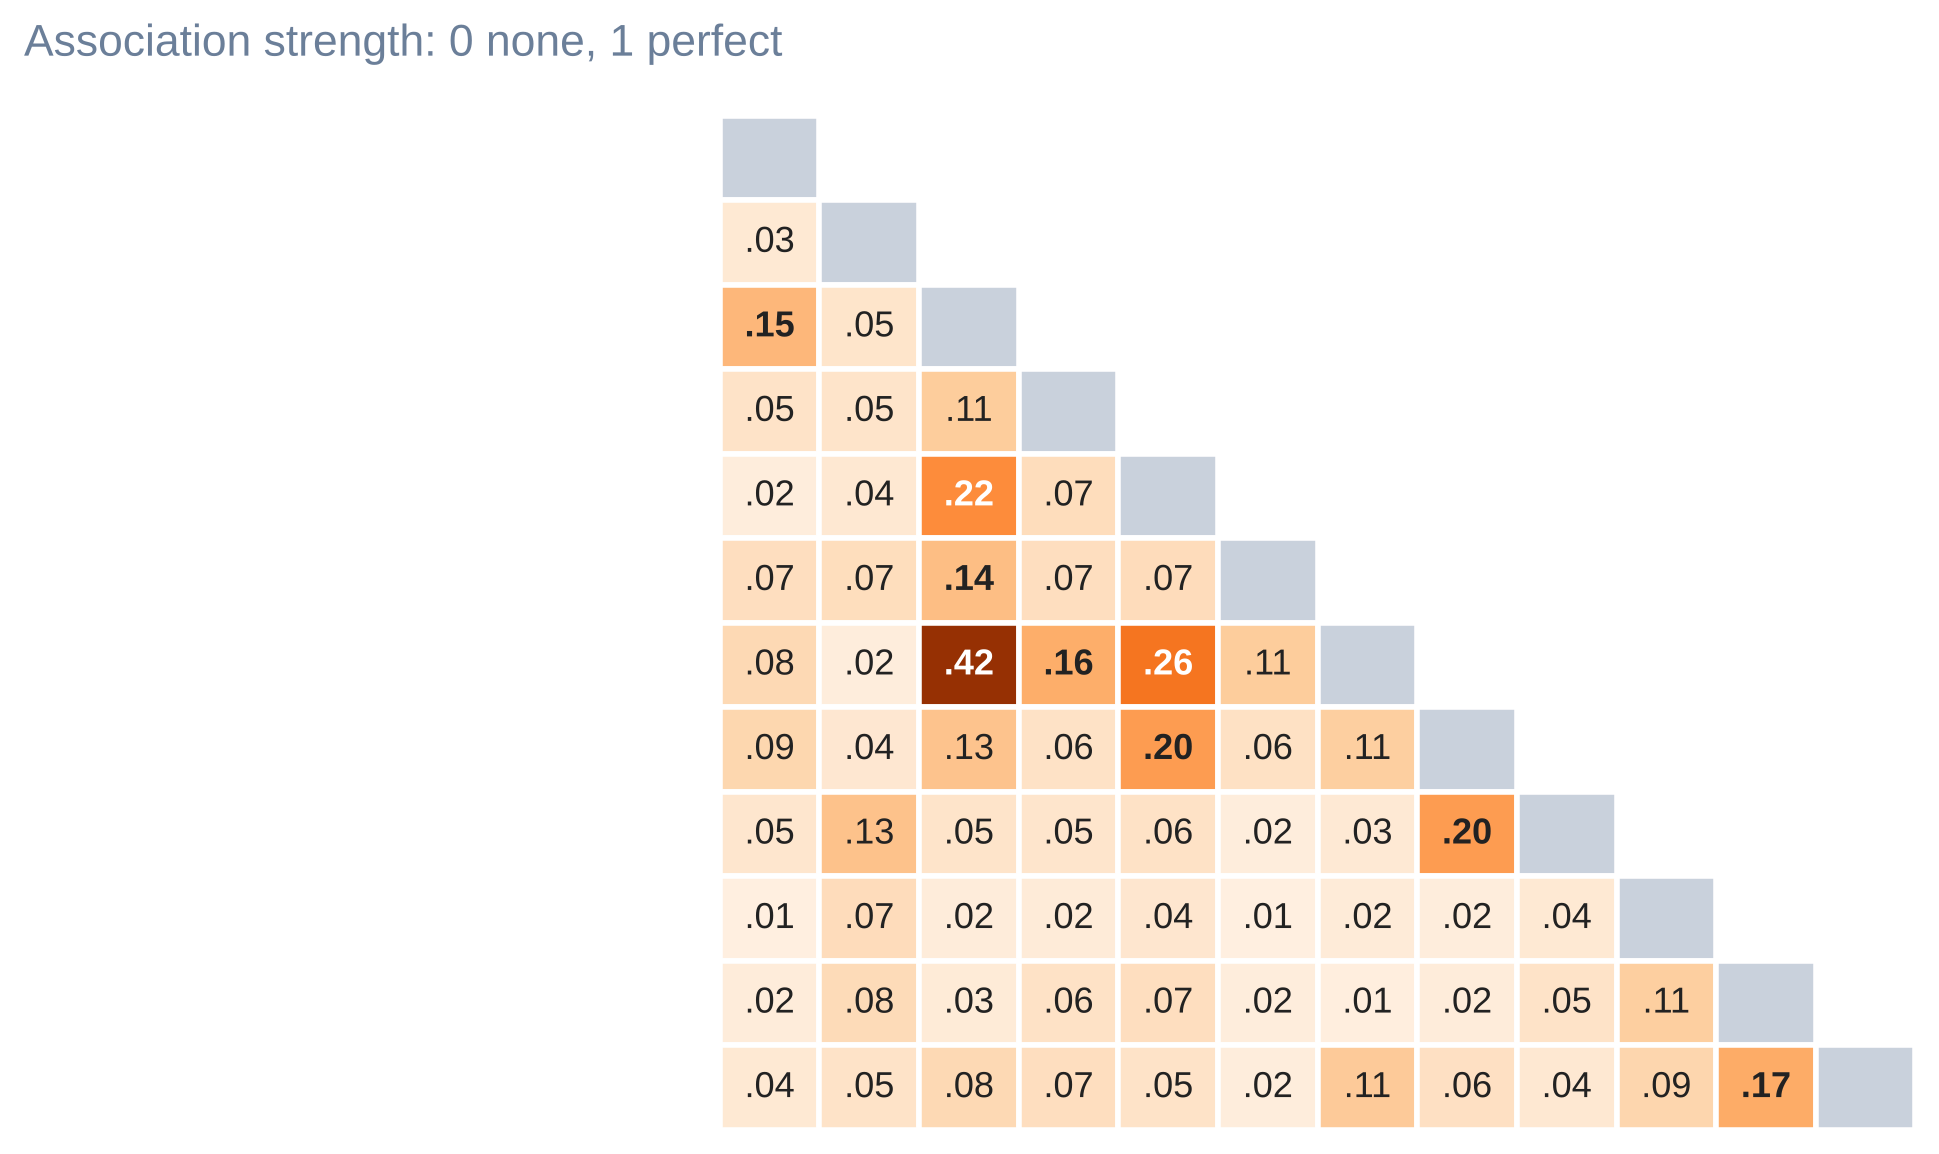
\includegraphics[width=0.86\textwidth]{f4_corr.png}
\caption{Association between each pair of variables (Cram\'er's $V$; 0 is none, 1 is perfect).}\label{fig:corr}
\end{figure}

\begin{figure}[htbp]
\centering
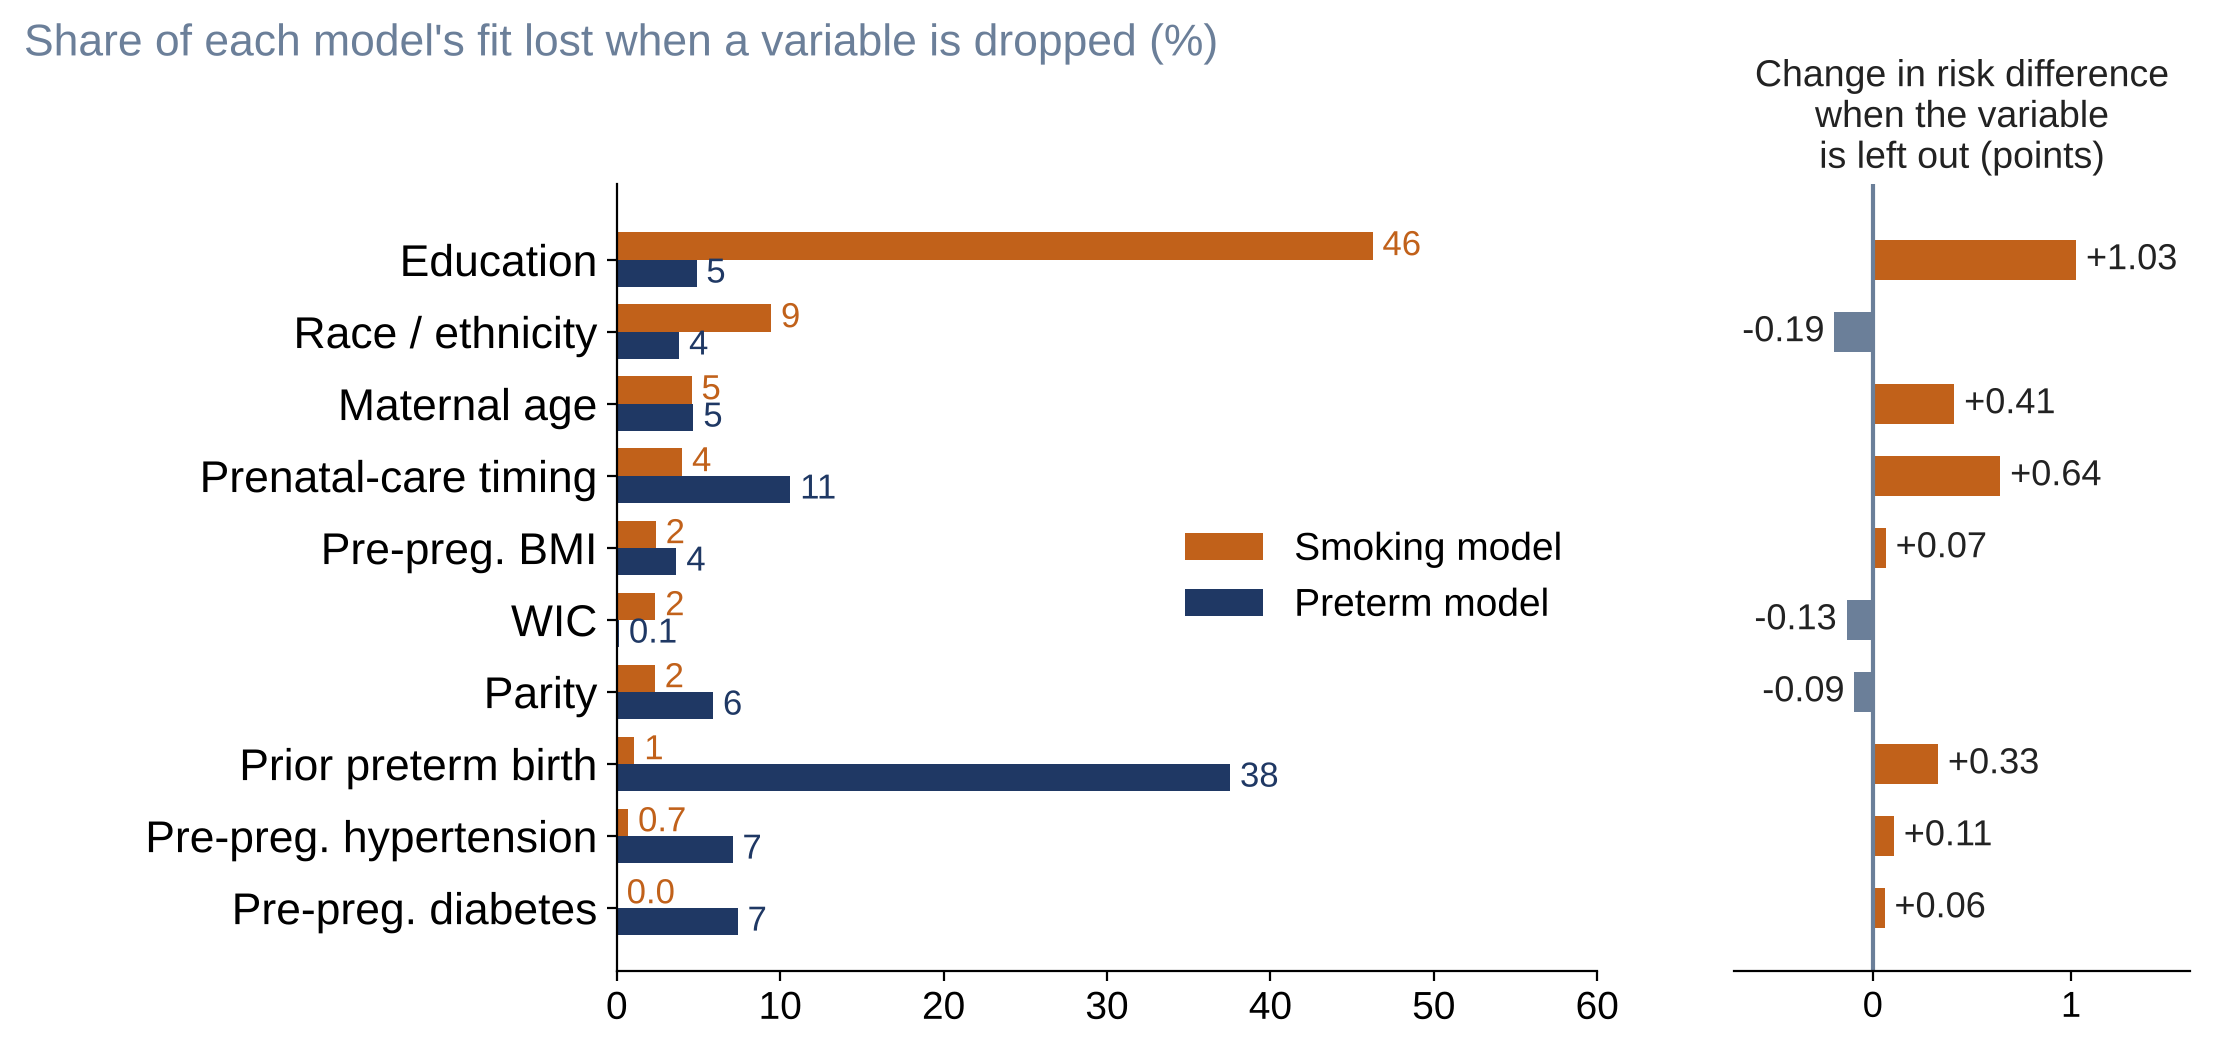
\includegraphics[width=\textwidth]{f5_rank.png}
\caption{Share of each model's fit lost when a variable is dropped (left) and change in the risk difference when that variable is left out of the adjustment set (right).}\label{fig:rank}
\end{figure}

\subsection*{Main estimate}
After AIPTW adjustment the risk difference was \RDmain{} points (bootstrap 95\% CI \BootLo{} to \BootHi{}), a risk ratio of \RRmain{} (Table~\ref{tab:main}). Adjustment reduced the crude difference by \ReducePct{}\%. Outcome regression gave \RDg{} and stabilized IPTW \RDiptw{} (\RDiptwLo{} to \RDiptwHi{}). Among mothers who smoked, the effect was \ATT{} points (\ATTlo{} to \ATThi{}), about \ExcessPerK{} additional preterm births per 1,000 smoking pregnancies, or \ExcessBirths{} births in this cohort if the assumptions hold.

\begin{table}[htbp]
\centering
\caption{Effect of smoking during pregnancy on preterm birth, risk difference in percentage points. Intervals are from the influence function; the bootstrap interval for the AIPTW estimate is \BootLo{} to \BootHi{}.}\label{tab:main}
{\small
\begin{tabular}{lrrr}
\toprule
Estimator & Risk difference (points) & 95\% CI & Risk ratio \\
\midrule
Crude (unadjusted) & 5.60 & 5.38 to 5.82 & 1.68 \\
Outcome regression (g-computation) & 3.48 &  &  \\
IPTW (stabilized) & 3.53 & 2.77 to 4.30 & 1.42 \\
AIPTW (doubly robust) & 3.26 & 2.47 to 4.04 & 1.39 \\
AIPTW, effect among smokers (ATT) & 3.39 & 3.17 to 3.61 &  \\
Overlap weights (ATO) & 3.30 & 3.08 to 3.52 & 1.32 \\
\bottomrule
\end{tabular}
}

\end{table}

\subsection*{Robustness to the adjustment set and propensity score rules}
The risk difference ranged from \RangeMin{} to \RangeMax{} points across all specifications (Table~\ref{tab:spec}, Fig.~\ref{fig:robust}). Removing prenatal-care timing and WIC gave \RDPre{} (\RDPreLo{} to \RDPreHi{}), a shift of \PreShift{} points, the largest change among the specifications examined. Without any clamping the estimate was \RDnoclamp{}, with a largest weight of \MaxWtNone{}, against \MaxWtClamp{} with clamping.

\begin{table}[htbp]
\centering
\caption{AIPTW risk difference under alternative covariate sets and propensity score rules.}\label{tab:spec}
{\small
\begin{tabular}{lrr}
\toprule
Analysis & Risk difference (points) & 95\% CI \\
\midrule
Crude, unadjusted & 5.60 & 5.38 to 5.82 \\
Main: ten confounders & 3.26 & 2.47 to 4.04 \\
Pre-pregnancy set only (no care timing, no WIC) & 3.65 & 2.88 to 4.43 \\
Main plus insurance type & 3.05 & 2.23 to 3.87 \\
Main plus two-way interactions & 3.02 & 2.46 to 3.59 \\
Clamp at 5 / 95 percentile & 3.22 & 2.72 to 3.72 \\
Overlap weights & 3.30 & 3.08 to 3.52 \\
Among smokers (ATT) & 3.39 & 3.17 to 3.61 \\
\bottomrule
\end{tabular}
}

\end{table}

\begin{figure}[htbp]
\centering
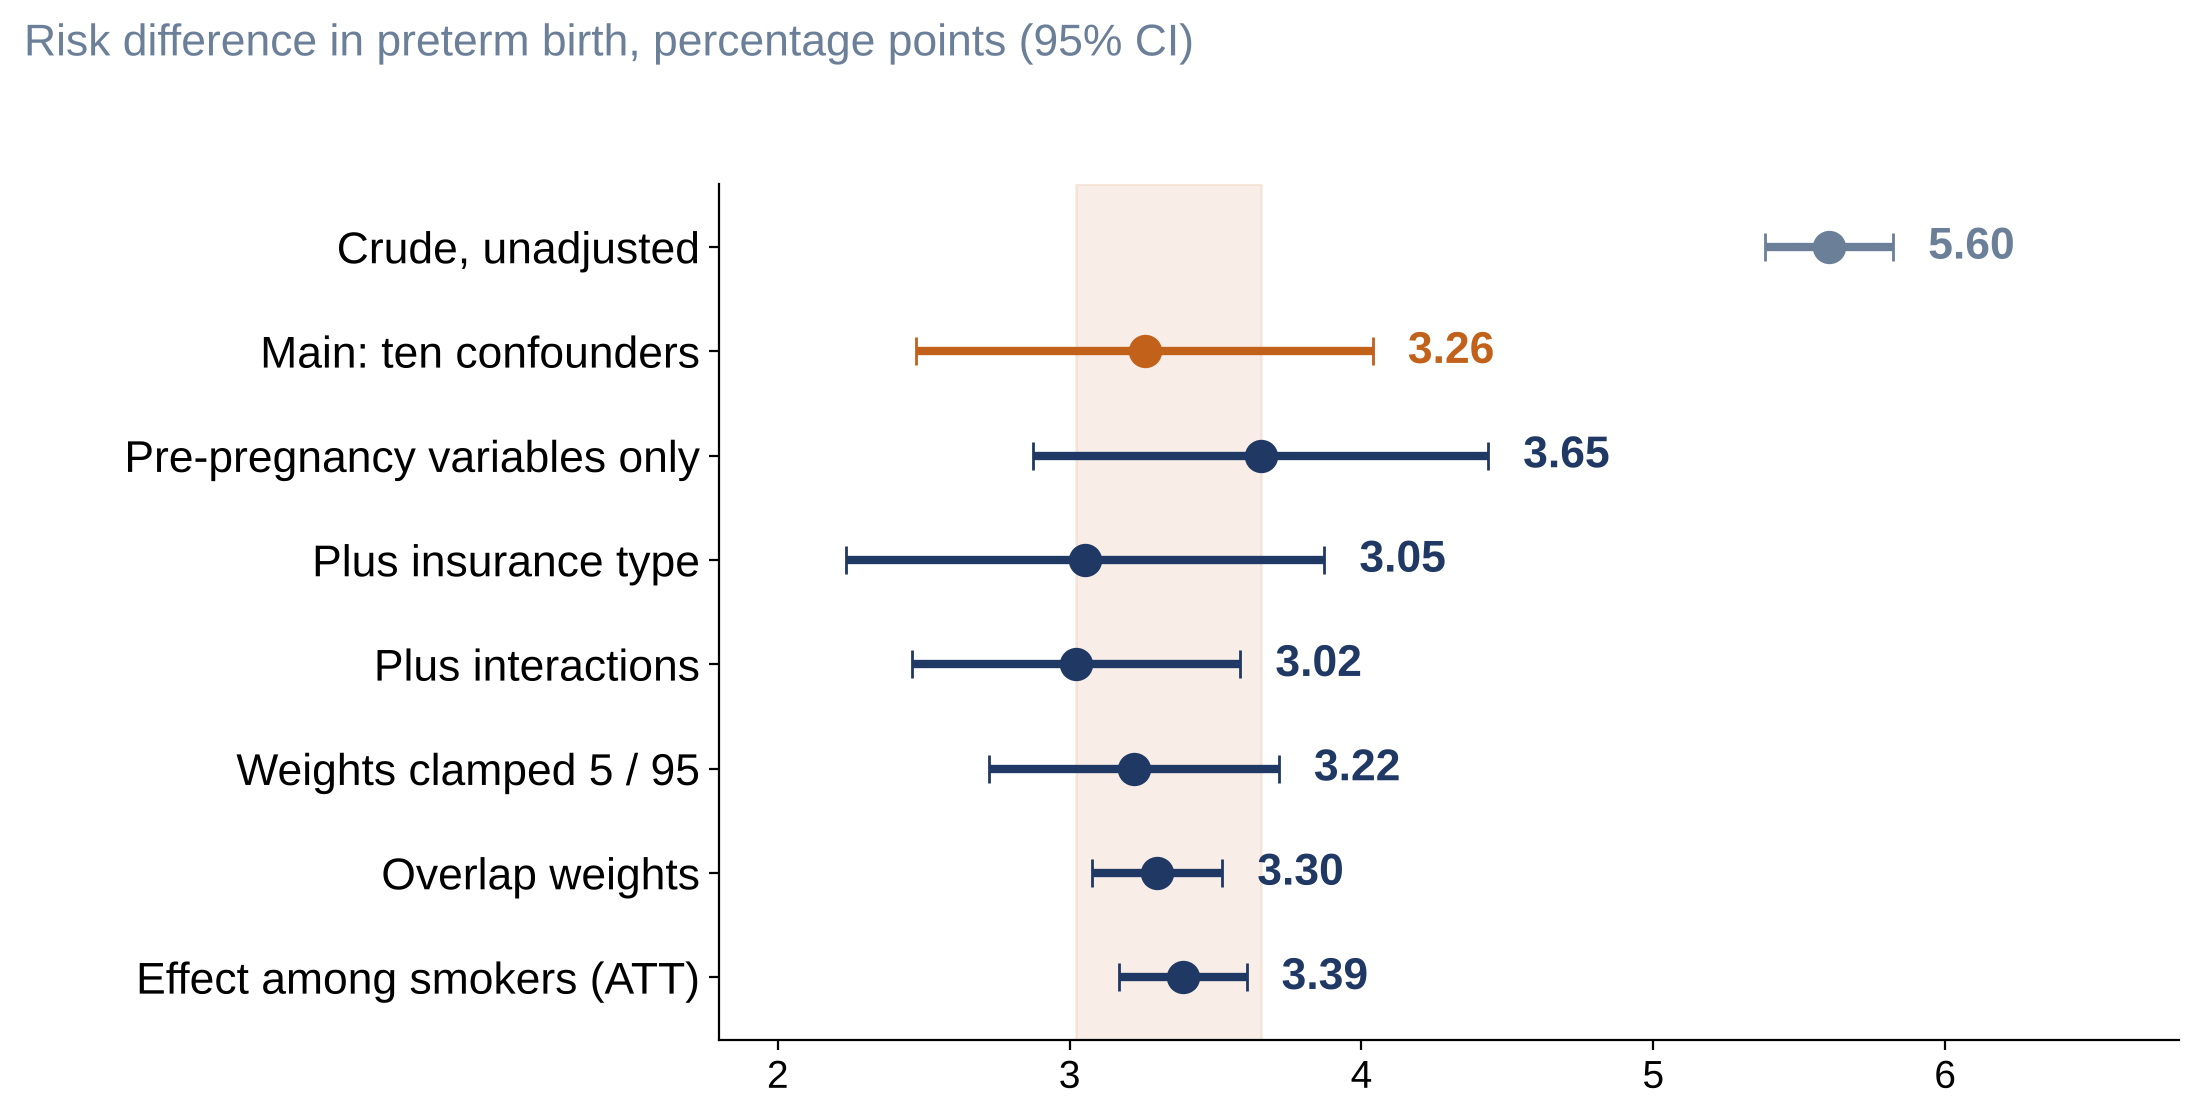
\includegraphics[width=0.9\textwidth]{f7_robust.png}
\caption{Risk difference in preterm birth (percentage points, 95\% CI) under alternative adjustment sets and weighting rules. The shaded band spans the adjusted estimates.}\label{fig:robust}
\end{figure}

\subsection*{Overlap and balance}
The propensity score separated the groups only partly (Fig.~\ref{fig:overlap}). \LowNon{}\% of non-smokers, but \LowSmk{}\% of smokers, had a score below 0.01, and \LowBachSum{}\% of the non-smokers in that low group held a bachelor's degree or higher, the group in which smoking is rare. The largest SMD fell from \SMDbefore{} before weighting to \SMDafter{} after IPTW (\BalAfter{} of \NLevels{} levels above 0.10, down from \BalBefore{}) and to \SMDov{} with overlap weights. The largest stabilized weight among smokers was \MaxWtClamp{} and the effective sample size of the weighted smokers was \ESSclamp{} of \NSmokers{}.

\begin{figure}[htbp]
\centering
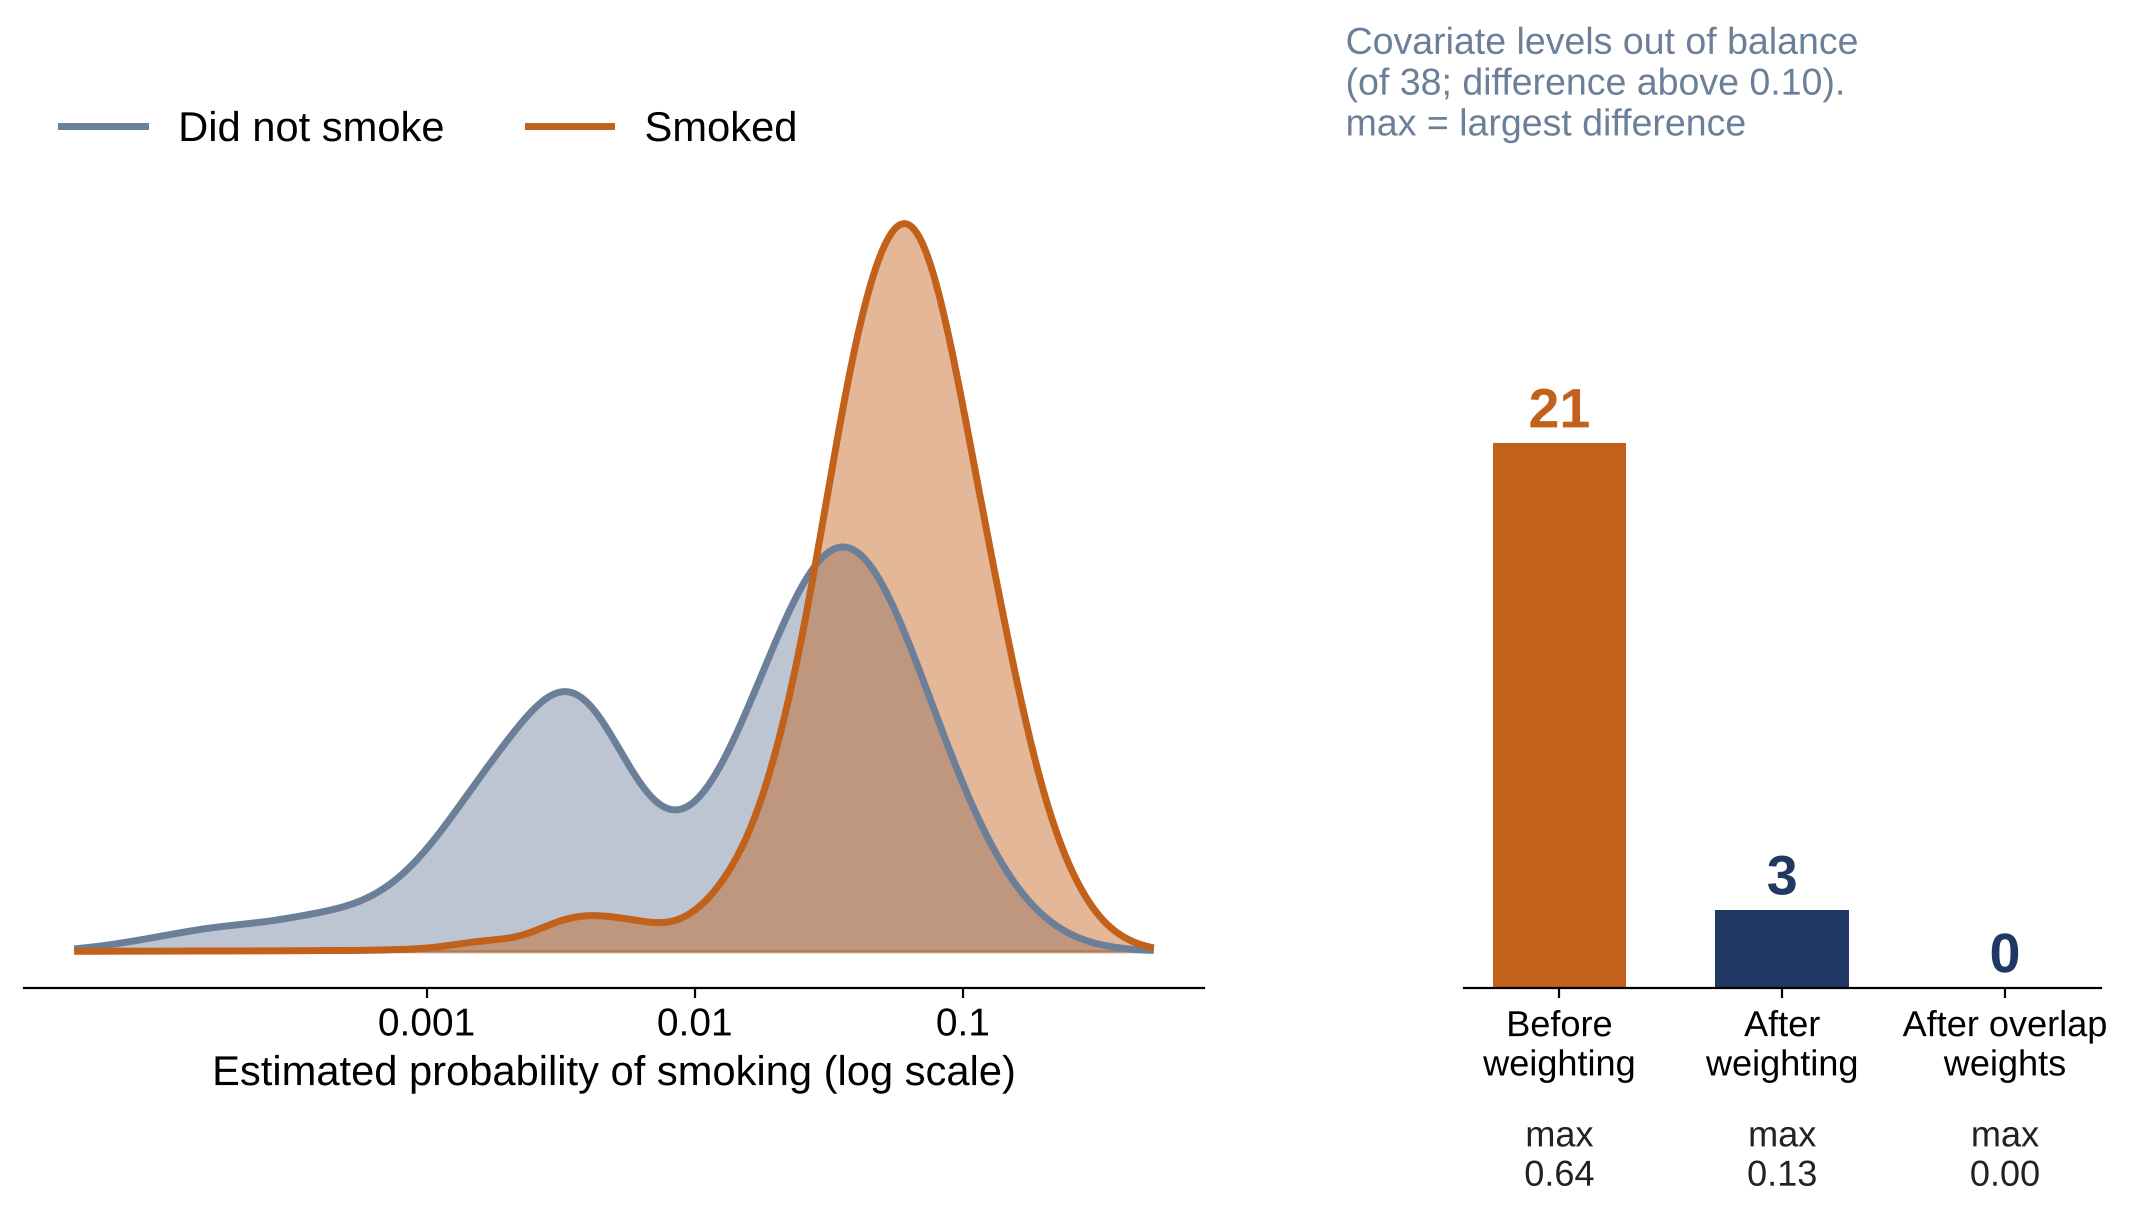
\includegraphics[width=0.95\textwidth]{f6_overlap.png}
\caption{Estimated probability of smoking by smoking status (left) and number of covariate levels with a standardized mean difference above 0.10 before and after weighting (right).}\label{fig:overlap}
\end{figure}

\subsection*{Variance}
The bootstrap standard error was \SEboot{} points (percentile 95\% CI \BootLo{} to \BootHi{}) against \SEif{} from the influence function, a ratio of \SEratio{} (Additional file 1, Table S3). The two are nearly identical, so the influence-function standard error is reliable here.

\subsection*{Flexible models with cross-fitting}
With cross-fitting, the risk difference was \CFLog{} with logistic regression, \CFLasso{} with LASSO and \CFForest{} with random forests; the average of the three was \CFAvg{} (Table~\ref{tab:cf}, Fig.~\ref{fig:flex}). The two random splits differed by at most \CFrange{} points. The forest gave the lowest estimate because its weights were more concentrated. Calibration of each learner is reported in Additional file 1 (Table S4).

\begin{table}[htbp]
\centering
\caption{Cross-fitted AIPTW with three learners (clamped at the 1st and 99th percentiles; mean of two random splits).}\label{tab:cf}
\resizebox{\textwidth}{!}{{\small
\begin{tabular}{lrrrrrr}
\toprule
Learner & Risk difference & 95\% CI & Outcome part & Weighting part & Largest weight & Effective n \\
\midrule
Logistic, main effects & 3.22 & 2.43 to 4.01 & 3.48 & 3.52 & 6,308 & 6,755 \\
LASSO with all two-way interactions & 2.80 & 2.02 to 3.57 & 3.85 & 3.01 & 6,922 & 6,428 \\
Random forest & 2.30 & 1.39 to 3.21 & 3.77 & 2.51 & 10,000 & 3,788 \\
Average of the three & 2.84 & 2.28 to 3.41 & 3.70 & 3.00 & 4,594 & 8,808 \\
\bottomrule
\end{tabular}
}
}
\end{table}

\begin{figure}[htbp]
\centering
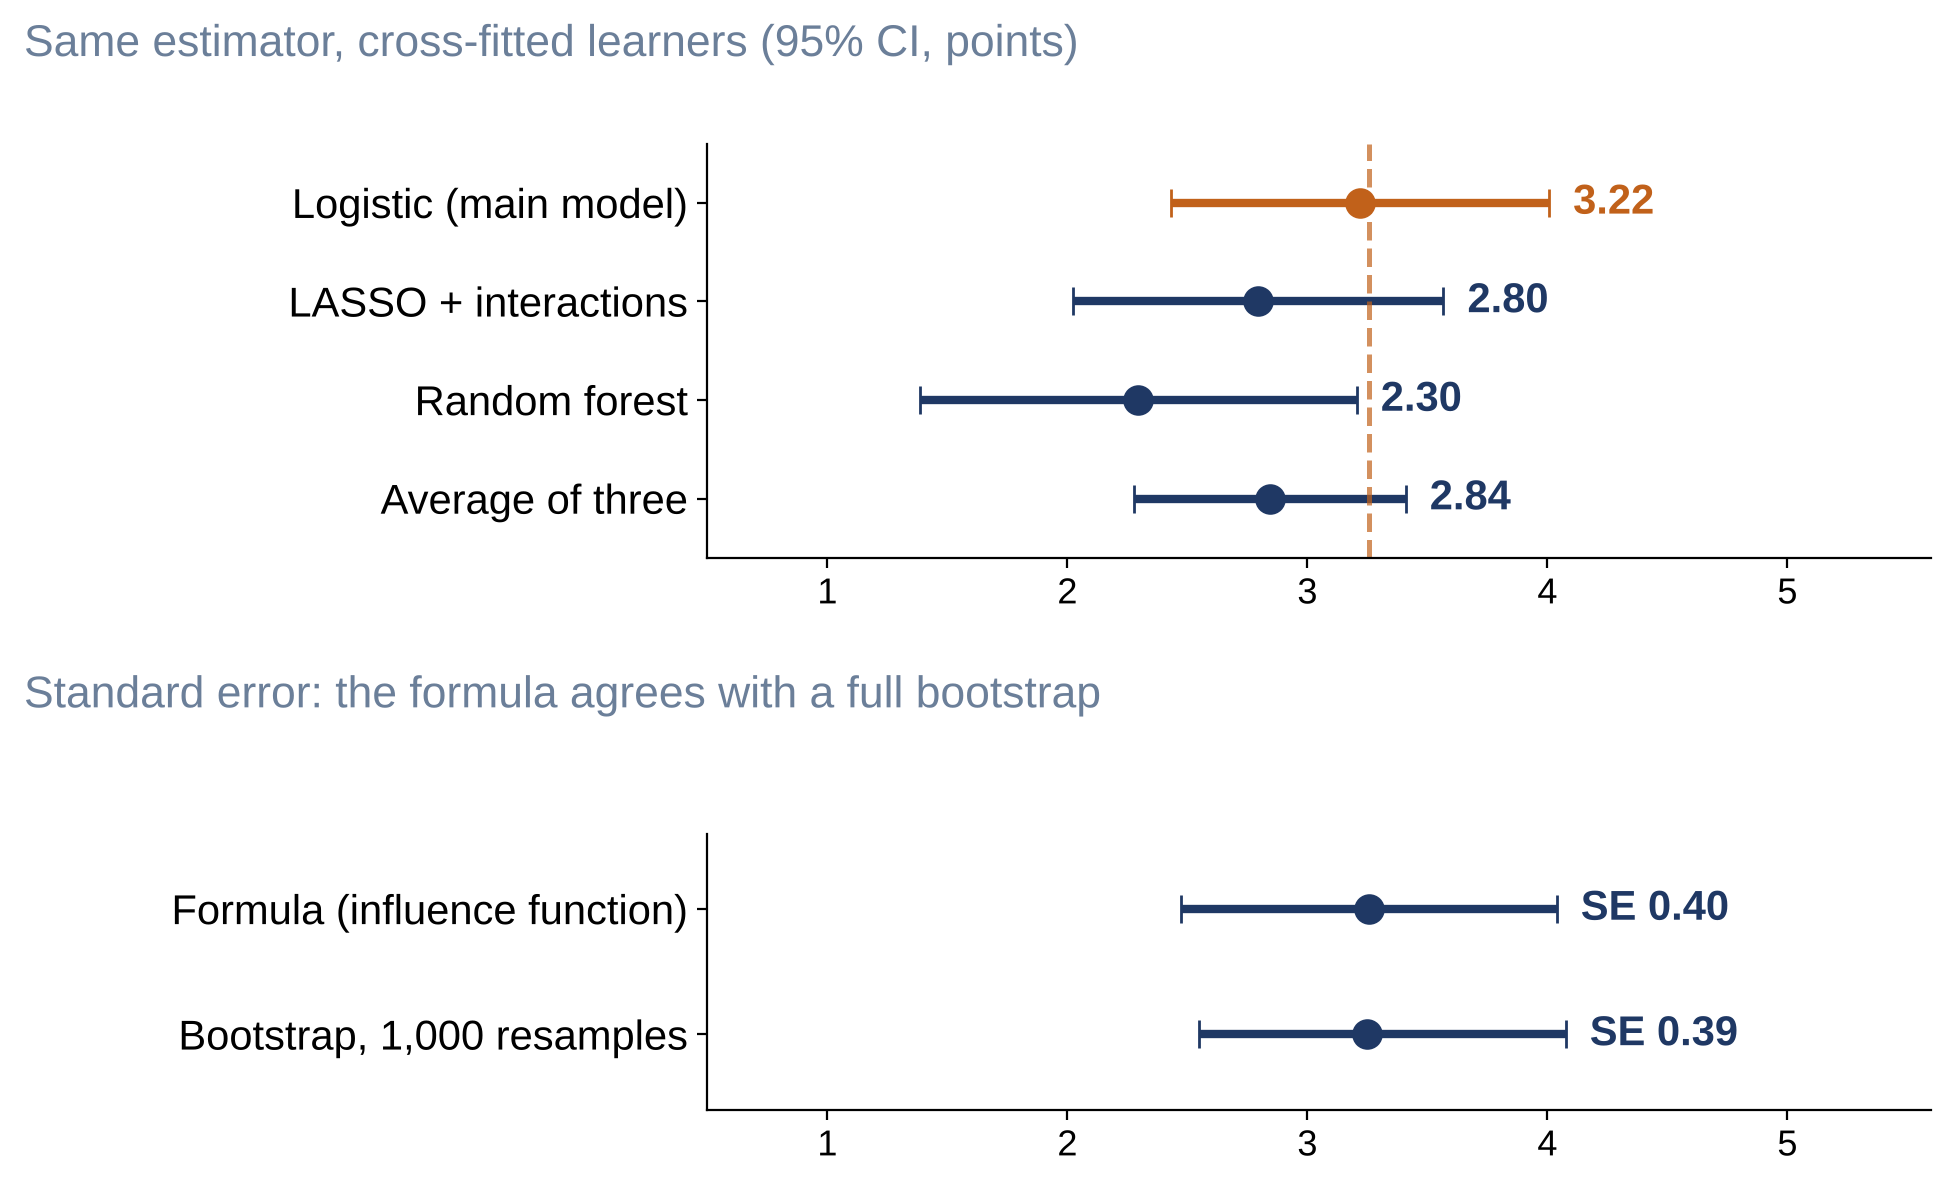
\includegraphics[width=0.95\textwidth]{f8_flex.png}
\caption{Cross-fitted risk difference by learner (top) and standard errors from the influence function and the full-sample bootstrap (bottom). The dashed line is the main estimate.}\label{fig:flex}
\end{figure}

\subsection*{Smoking history and intensity (exploratory)}
Crude preterm risk was \HistNever{}\% in mothers who never smoked, \HistQuit{}\% in those who quit, \HistCont{}\% in those who continued and \HistStart{}\% in those who started during pregnancy (Additional file 1, Table S5). Comparing continuers with quitters, adjusted for the confounders and pre-pregnancy intensity, gave \ContQuit{} points (\ContQuitLo{} to \ContQuitHi{}). Quitters compared with never-smokers differed by $\QuitNever$ points among quitters ($\QuitNeverLo$ to \QuitNeverHi{}) (Fig.~\ref{fig:cess}). Among mothers who continued, the effect was similar at every pre-pregnancy cigarette level (\DoseMin{} to \DoseMax{} points).

\begin{figure}[htbp]
\centering
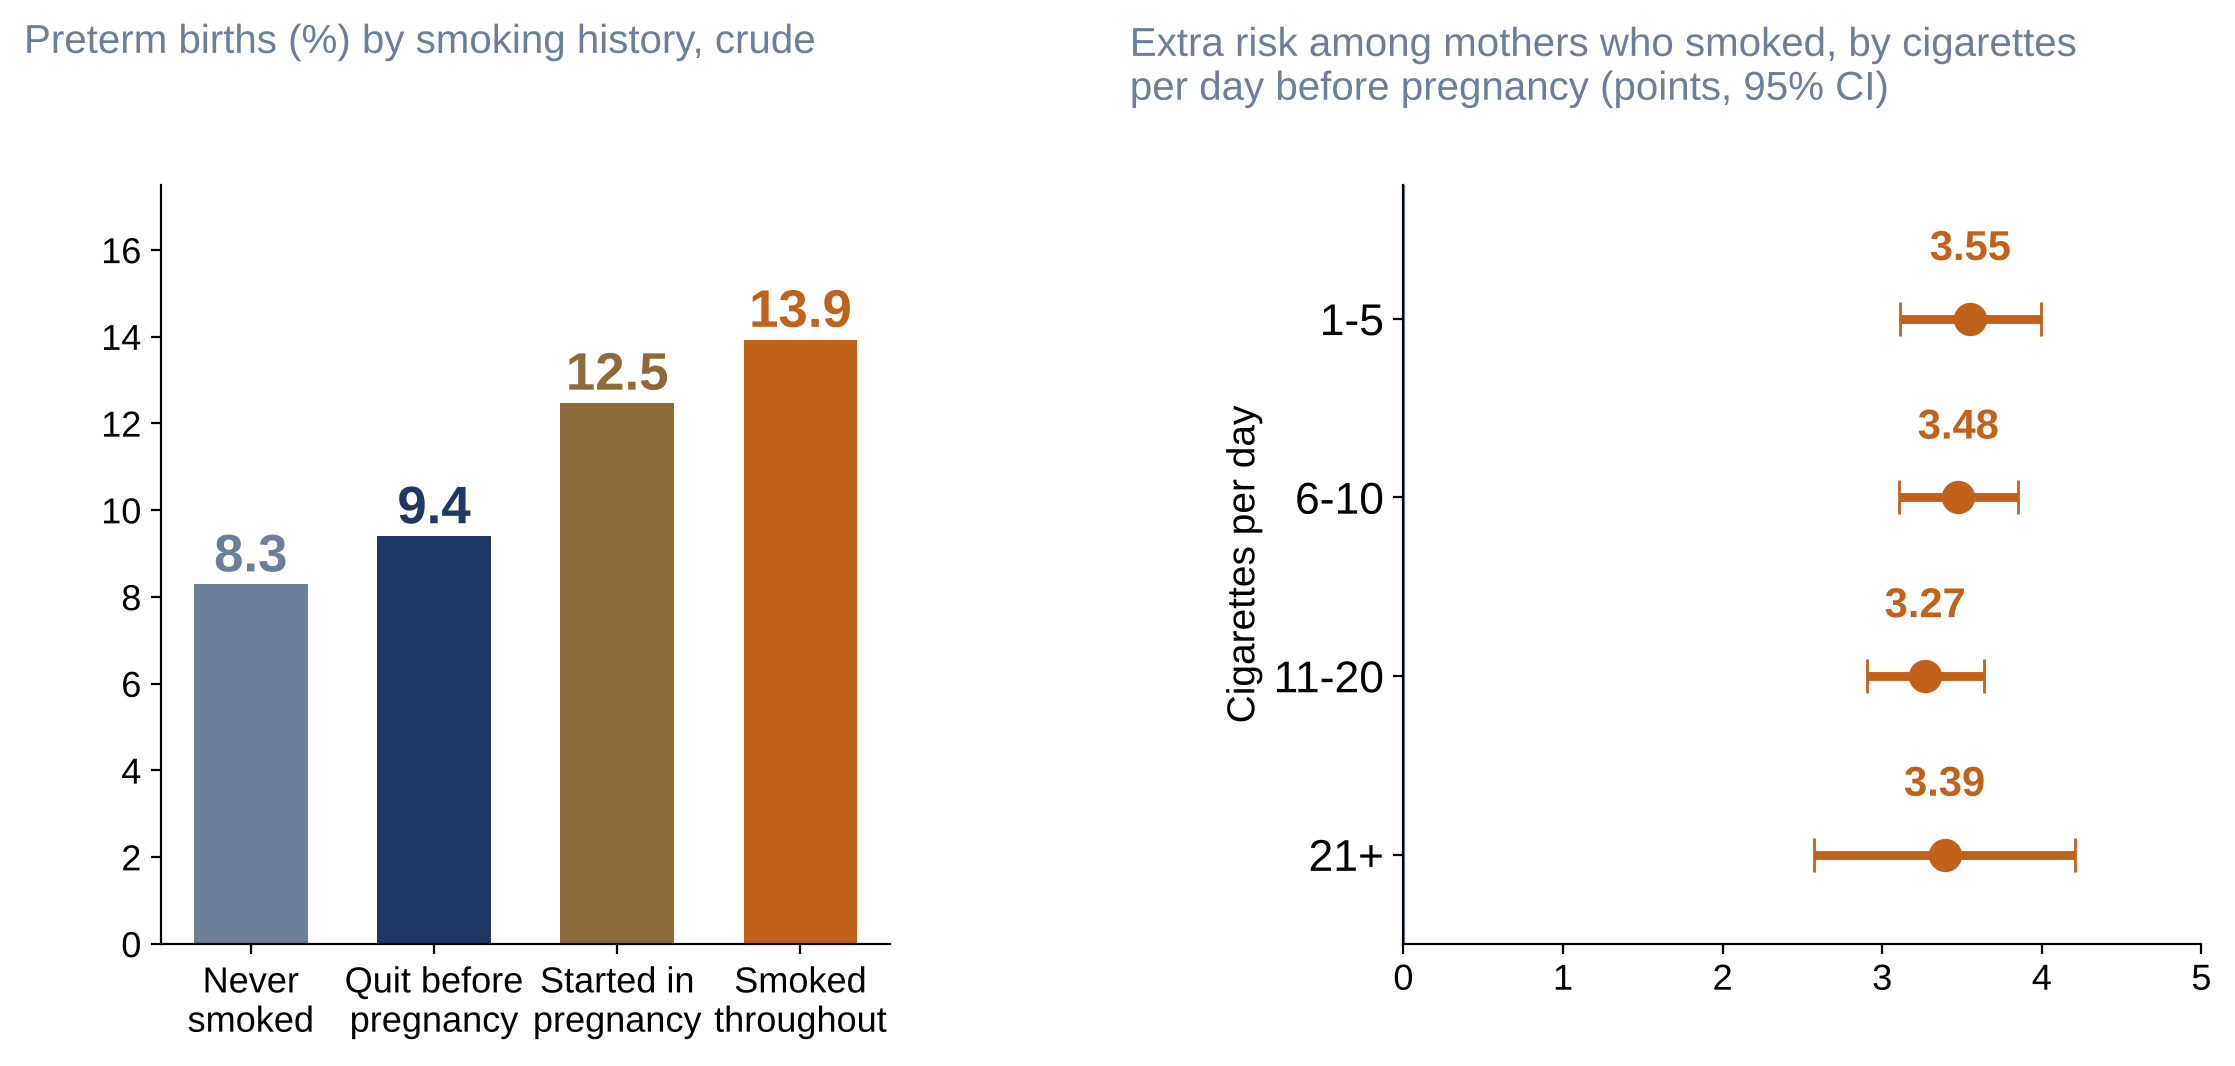
\includegraphics[width=\textwidth]{f9_cess.png}
\caption{Preterm births by smoking history (left) and effect among mothers who smoked by cigarettes per day before pregnancy (right; points, 95\% CI).}\label{fig:cess}
\end{figure}

\subsection*{Trimester of smoking (exploratory)}
Rebuilding the cohort from the full national file gave the same \NTotal{} births, and \TriN{} of them had known cigarettes in every period. Crude preterm risk was \TriNever{}\% in the reference group, \TriFirst{}\% in mothers who smoked in the first trimester only, \TriFirstSecond{}\% in the first and second trimesters only, \TriAll{}\% in all three trimesters and \TriLate{}\% in those who started after the first trimester (Table~\ref{tab:tri}). After adjustment, the effect among those who smoked was \TriAATT{} points (\TriALo{} to \TriAHi{}) for the first trimester only, \TriBATT{} (\TriBLo{} to \TriBHi{}) for the first and second trimesters and \TriCATT{} (\TriCLo{} to \TriCHi{}) for all three. The \TriLateN{} mothers who started after the first trimester gave \TriDATT{} points (\TriDLo{} to \TriDHi{}), too imprecise to interpret. Among mothers who smoked in all three trimesters the effect rose with third-trimester intensity: \TriDoseA{}, \TriDoseB{}, \TriDoseC{} and \TriDoseD{} points at 1 to 5, 6 to 10, 11 to 20 and 21 or more cigarettes per day. As in the pre-pregnancy intensity analysis, the whole-population estimate for the smallest group is unstable (\TriDoseWideATE{} points, \TriDoseWideLo{} to \TriDoseWideHi{} for 21 or more), so the effect among smokers is the reading to use.

\begin{table}[htbp]
\centering
\caption{Trimester of smoking and third-trimester intensity, each group against mothers who never smoked (full 2023 natality file; risk difference in percentage points).}\label{tab:tri}
\resizebox{\textwidth}{!}{{\small
\begin{tabular}{lrrrrrr}
\toprule
Smoking pattern, each against never-smokers & Group size & Crude & ATE & 95\% CI & ATT & 95\% CI \\
\midrule
First trimester only & 13,215 & 2.79 & 2.07 & 1.05 to 3.10 & 1.38 & 0.86 to 1.90 \\
First and second trimesters only & 5,366 & 5.23 & 3.53 & 1.65 to 5.41 & 3.43 & 2.55 to 4.31 \\
All three trimesters & 74,962 & 5.98 & 3.46 & 2.18 to 4.74 & 3.68 & 3.43 to 3.93 \\
Started after the first trimester & 2,288 & 2.81 & 1.08 & $-$1.94 to 4.09 & 0.87 & $-$0.36 to 2.11 \\
All three trimesters, 1-5 cigarettes/day in 3rd trimester & 32,137 & 5.42 & 2.97 & 1.61 to 4.32 & 3.26 & 2.89 to 3.63 \\
All three trimesters, 6-10 cigarettes/day in 3rd trimester & 27,813 & 6.00 & 4.50 & 1.05 to 7.94 & 3.72 & 3.32 to 4.12 \\
All three trimesters, 11-20 cigarettes/day in 3rd trimester & 13,447 & 7.03 & 2.41 & 0.18 to 4.64 & 4.44 & 3.85 to 5.03 \\
All three trimesters, 21+ cigarettes/day in 3rd trimester & 1,565 & 8.16 & 11.02 & $-$2.17 to 24.20 & 5.03 & 3.26 to 6.80 \\
\bottomrule
\end{tabular}
}
}
\end{table}

\subsection*{Unmeasured confounding}
The E-value for the point estimate was \EV{} and for the lower confidence limit \EVlo{}. Previous preterm birth, the strongest measured predictor of preterm birth, is the only measured level whose association with both smoking (risk ratio 2.42) and preterm birth (3.42) exceeds the E-value, and omitting it moves the estimate by only \PPChange{} points (Additional file 1, Table S6).

\section*{Discussion}

In 2023 U.S. singleton births, smoking during pregnancy raised the risk of preterm birth by about \RDmain{} percentage points (risk ratio \RRmain{}) under the stated assumptions, which is \ReducePct{}\% less than the crude difference. The adjusted marginal odds ratio of 1.44 lies inside the 1.31 to 1.53 range reported for first-trimester smoking by cigarettes per day in a regression analysis of 25.6 million births \cite{liu2020}. Among mothers who smoked, the effect translates to about \OneIn{} smoking pregnancies for each additional preterm birth, which gives health departments a count to use when comparing cessation programs.

Four findings support the stability of the result. The standard error did not change materially when the whole pipeline was resampled. The estimate moved little when the nuisance models were flexible and cross-fitted. It stayed within \RangeMin{} to \RangeMax{} points across specifications. And the overlap-weighted estimate, which targets mothers with comparable counterparts, was \ATO{} points. The effect among smokers was smaller for mothers who smoked only in the first trimester (\TriAATT{} points) than for those who smoked in all three (\TriCATT{} points), in line with a benefit of stopping early, and mothers who quit before pregnancy resembled mothers who never smoked. Both findings are exploratory. The time a mother can smoke is limited by when she delivers, so the shorter-exposure groups contain early deliveries by construction, and these comparisons describe patterns of reported smoking and not the effect of stopping at a chosen time.

\subsection*{Strengths and limitations}
The study uses a national file of 3.26 million births, states each identifying assumption (Table~\ref{tab:assump}), reports an absolute effect, and examines overlap, variance, model flexibility and unmeasured confounding in one framework.

Smoking is self-reported on the birth certificate and is underreported \cite{dietz2011,howland2015,searles2014}. Non-differential misclassification of a binary exposure usually biases toward the null \cite{jurek2005}. Overlap is limited: \LowNon{}\% of non-smokers have a score below 0.01, concentrated among mothers with a college degree, so the ATE depends on few smokers with large weights. The ATT, which needs weights only for non-smokers, and the overlap-weighted estimate are less affected. Prenatal-care timing and WIC may follow smoking, and the estimate without them was \RDPre{}. Complete-case analysis excluded \NDropped{} births, whose preterm risk was higher (\DroppedPreterm{}\% against \KeptPreterm{}\%). The file contains live births only \cite{leung2021}. Alcohol, cannabis, e-cigarettes, stress and interpregnancy interval are unmeasured \cite{patra2011,regan2021}. ``Any smoking'' averages over dose and timing. The results are for one national year.

\section*{Conclusions}
In \NTotal{} singleton births, the AIPTW risk difference for preterm birth was \RDmain{} percentage points (95\% bootstrap CI \BootLo{} to \BootHi{}), \ATT{} points among mothers who smoked. The estimate was stable across the bootstrap, flexible learners and changes to the adjustment set. It rests on limited overlap, self-reported smoking and assumptions that the E-value quantifies but cannot verify.

\section*{Abbreviations}
\textit{AIPTW}: augmented inverse probability of treatment weighting; \textit{ATE}: average treatment effect; \textit{ATT}: average treatment effect among the treated; \textit{BMI}: body mass index; \textit{CI}: confidence interval; \textit{NCHS}: National Center for Health Statistics; \textit{SMD}: standardized mean difference; \textit{WIC}: Special Supplemental Nutrition Program for Women, Infants, and Children.

\section*{Declarations}
\textbf{Ethics approval and consent to participate.} Not applicable. The study analysed a public-use file with no personal identifiers.

\textbf{Consent for publication.} Not applicable.

\textbf{Availability of data and materials.} The data are the public-use 2023 Natality file of the National Center for Health Statistics (\url{https://ftp.cdc.gov/pub/Health_Statistics/NCHS/Datasets/DVS/natality/Nat2023us.zip}). The analysis extract, the compact trimester file and the R script that produces every number and figure are available at \url{https://github.com/fmurital/Causal-Inference-}. The script reads the data directly from that repository.

\textbf{Competing interests.} The authors declare that they have no competing interests.

\textbf{Funding.} No external funding was received for this study.

\textbf{Authors' contributions.} FM conceived the question, designed and carried out the analysis and drafted the manuscript. DG supervised the work and revised the manuscript. Both authors read and approved the final manuscript.

\textbf{Acknowledgements.} Not applicable.

\textbf{Use of AI assistance.} The authors used an AI assistant (Claude, Anthropic) to organize the literature, to help write and test the R code, and to draft and edit text. The first author specified the question, the design and the analytic choices and ran the code, and the numbers come directly from the code output. Both authors are responsible for the content.

\section*{References}
{\small\begin{enumerate}[leftmargin=2.4em,labelsep=0.4em,itemsep=2pt,parsep=0pt,label={\arabic*.}]
\item Martin JA, Hamilton BE, Osterman MJK. Births in the United States, 2023. NCHS Data Brief No. 507. Hyattsville, MD: National Center for Health Statistics; 2024. \url{https://doi.org/10.15620/cdc/158789}
\item Martin JA, Osterman MJK, Driscoll AK. Declines in cigarette smoking during pregnancy in the United States, 2016-2021. NCHS Data Brief No. 458. Hyattsville, MD: National Center for Health Statistics; 2023.
\item Liu B, Xu G, Sun Y, Qiu X, Ryckman KK, Yu Y, et al. Maternal cigarette smoking before and during pregnancy and the risk of preterm birth: a dose-response analysis of 25 million mother-infant pairs. PLoS Med. 2020;17(8):e1003158. \url{https://doi.org/10.1371/journal.pmed.1003158}
\item Stock SJ, Bauld L. Maternal smoking and preterm birth: an unresolved health challenge. PLoS Med. 2020;17(9):e1003386. \url{https://doi.org/10.1371/journal.pmed.1003386}
\item Kondracki AJ. Low birthweight in term singletons mediates the association between maternal smoking intensity exposure status and immediate neonatal intensive care unit admission: the E-value assessment. BMC Pregnancy Childbirth. 2020. \url{https://doi.org/10.1186/s12884-020-02981-1}
\item Bang H, Robins JM. Doubly robust estimation in missing data and causal inference models. Biometrics. 2005;61(4):962-73. \url{https://doi.org/10.1111/j.1541-0420.2005.00377.x}
\item Chernozhukov V, Chetverikov D, Demirer M, Duflo E, Hansen C, Newey W, et al. Double/debiased machine learning for treatment and structural parameters. Econom J. 2018;21(1):C1-68. \url{https://doi.org/10.1111/ectj.12097}
\item VanderWeele TJ, Ding P. Sensitivity analysis in observational research: introducing the E-value. Ann Intern Med. 2017;167(4):268-74. \url{https://doi.org/10.7326/M16-2607}
\item National Center for Health Statistics. User guide to the 2023 natality public use file. Hyattsville, MD: NCHS; 2024. \url{https://ftp.cdc.gov/pub/Health_Statistics/NCHS/Dataset_Documentation/DVS/natality/UserGuide2023.pdf}
\item Martin JA, Osterman MJK, Kirmeyer SE, Gregory ECW. Measuring gestational age in vital statistics data: transitioning to the obstetric estimate. Natl Vital Stat Rep. 2015;64(5).
\item Tennant PWG, Murray EJ, Arnold KF, Berrie L, Fox MP, Gadd SC, et al. Use of directed acyclic graphs (DAGs) to identify confounders in applied health research: review and recommendations. Int J Epidemiol. 2021;50(2):620-32. \url{https://doi.org/10.1093/ije/dyaa213}
\item Pearl J. Causal diagrams for empirical research. Biometrika. 1995;82(4):669-88. \url{https://doi.org/10.1093/biomet/82.4.669}
\item Shin D, Song WO. Influence of the adequacy of the Prenatal Care Utilization Index on small-for-gestational-age infants and preterm births in the United States. J Clin Med. 2019;8(6):838. \url{https://doi.org/10.3390/jcm8060838}
\item Joyce T, Racine A, Yunzal-Butler C. Reassessing the WIC effect: evidence from the Pregnancy Nutrition Surveillance System. J Policy Anal Manage. 2008;27(2):277-303.
\item Heaman MI, Newburn-Cook CV, Green CG, Elliott LJ, Helewa ME. Inadequate prenatal care and its association with adverse pregnancy outcomes: a comparison of indices. BMC Pregnancy Childbirth. 2008;8:15.
\item Rubin DB. Estimating causal effects of treatments in randomized and nonrandomized studies. J Educ Psychol. 1974;66(5):688-701.
\item Rosenbaum PR, Rubin DB. The central role of the propensity score in observational studies for causal effects. Biometrika. 1983;70(1):41-55. \url{https://doi.org/10.1093/biomet/70.1.41}
\item Hern\'an MA, Robins JM. Causal inference: what if. Boca Raton: Chapman \& Hall/CRC; 2020.
\item Cole SR, Frangakis CE. The consistency statement in causal inference: a definition or an assumption? Epidemiology. 2009;20(1):3-5. \url{https://doi.org/10.1097/EDE.0b013e31818ef366}
\item Petersen ML, Porter KE, Gruber S, Wang Y, van der Laan MJ. Diagnosing and responding to violations in the positivity assumption. Stat Methods Med Res. 2012;21(1):31-54. \url{https://doi.org/10.1177/0962280210386207}
\item Funk MJ, Westreich D, Wiesen C, St\"urmer T, Brookhart MA, Davidian M. Doubly robust estimation of causal effects. Am J Epidemiol. 2011;173(7):761-7. \url{https://doi.org/10.1093/aje/kwq439}
\item Li F, Morgan KL, Zaslavsky AM. Balancing covariates via propensity score weighting. J Am Stat Assoc. 2018;113(521):390-400. \url{https://doi.org/10.1080/01621459.2016.1260466}
\item Zivich PN, Breskin A. Machine learning for causal inference: on the use of cross-fit estimators. Epidemiology. 2021;32(3):393-401. \url{https://doi.org/10.1097/EDE.0000000000001332}
\item Austin PC, Stuart EA. Moving towards best practice when using inverse probability of treatment weighting (IPTW) using the propensity score to estimate causal treatment effects in observational studies. Stat Med. 2015;34(28):3661-79. \url{https://doi.org/10.1002/sim.6607}
\item Dietz PM, Homa D, England LJ, Burley K, Tong VT, Dube SR, et al. Estimates of nondisclosure of cigarette smoking among pregnant and nonpregnant women of reproductive age in the United States. Am J Epidemiol. 2011;173(3):355-9. \url{https://doi.org/10.1093/aje/kwq381}
\item Howland RE, Mulready-Ward C, Madsen AM, Sackoff J, Nyland-Funke M, Bombard JM, et al. Reliability of reported maternal smoking: comparing the birth certificate to maternal worksheets and prenatal and hospital medical records, New York City and Vermont, 2009. Matern Child Health J. 2015;19(9):1916-24. \url{https://doi.org/10.1007/s10995-015-1722-1}
\item Searles Nielsen S, Dills RL, Glass M, Mueller BA. Accuracy of prenatal smoking data from Washington State birth certificates in a population-based sample with cotinine measurements. Ann Epidemiol. 2014;24(3). \url{https://doi.org/10.1016/j.annepidem.2013.12.008}
\item Jurek AM, Greenland S, Maldonado G, Church TR. Proper interpretation of non-differential misclassification effects: expectations vs observations. Int J Epidemiol. 2005;34(3):680-7. \url{https://doi.org/10.1093/ije/dyi060}
\item Leung M, Kioumourtzoglou MA, Raz R, Weisskopf MG. Bias due to selection on live births in studies of environmental exposures during pregnancy: a simulation study. Environ Health Perspect. 2021;129(4):047001. \url{https://doi.org/10.1289/EHP7961}
\item Patra J, Bakker R, Irving H, Jaddoe VWV, Malini S, Rehm J. Dose-response relationship between alcohol consumption before and during pregnancy and the risks of low birthweight, preterm birth and small for gestational age (SGA): a systematic review and meta-analyses. BJOG. 2011;118(12):1411-21. \url{https://doi.org/10.1111/j.1471-0528.2011.03050.x}
\item Regan AK, Bombard JM, O'Hegarty MM, Smith RA, Tong VT. Adverse birth outcomes associated with prepregnancy and prenatal electronic cigarette use. Obstet Gynecol. 2021;138(1):85-94. \url{https://doi.org/10.1097/AOG.0000000000004432}
\end{enumerate}}


\clearpage
\setcounter{table}{0}\renewcommand{\thetable}{S\arabic{table}}
\section*{Additional file 1}
{\centering\captionof{table}{Analysis variables: how each is stored, its levels and missing values.}\par}
{\small
\begin{longtable}{llrp{7.2cm}r}
\toprule
Variable & Stored as & Levels & Levels or range & \% missing \\
\midrule
\endhead
\texttt{smoker} & integer &  & 0 to 1 & 0.00 \\
\texttt{preterm} & integer &  & 0 to 1 & 0.00 \\
\texttt{ga\_weeks} & integer &  & 17 to 47 & 0.00 \\
\texttt{mager} & integer &  & 12 to 50 & 0.00 \\
\texttt{age\_grp} & factor & 6 & $<$20 | 20-24 | 25-29 | 30-34 | 35-39 | 40+ & 0.00 \\
\texttt{race} & factor & 6 & White | Black | AIAN | Asian | NHOPI | Multiracial & 0.00 \\
\texttt{educ} & factor & 8 & $<$9th grade | 9-12th, no diploma | HS grad/GED | Some college | Associate | Bachelor's | Master's | Doctorate/Prof. & 1.69 \\
\texttt{precare} & factor & 4 & 1st trimester | 2nd trimester | 3rd trimester | No care & 1.78 \\
\texttt{wic} & factor & 2 & No | Yes & 0.98 \\
\texttt{parity} & factor & 4 & 0 | 1 | 2 | 3+ & 0.22 \\
\texttt{ppterm} & factor & 2 & No | Yes & 0.13 \\
\texttt{pdiab} & factor & 2 & No | Yes & 0.13 \\
\texttt{phype} & factor & 2 & No | Yes & 0.13 \\
\texttt{bmi} & numeric &  & 13 to 69.9 & 2.16 \\
\texttt{bmi\_grp} & factor & 6 & $<$18.5 | 18.5-24.9 | 25-29.9 | 30-34.9 | 35-39.9 | 40+ & 2.16 \\
\texttt{pay} & factor & 5 & Medicaid | Private | Self-pay | Other | Unknown & 0.00 \\
\texttt{cig\_0} & integer &  & 0 to 99 & 0.00 \\
\bottomrule
\end{longtable}
}
\addtocounter{table}{-1}\clearpage
\begin{table}[htbp]\centering\caption{Births in the cohort compared with births dropped for missing confounders.}{\small
\begin{tabular}{lrrr}
\toprule
Group & Births & \% smoked & \% preterm \\
\midrule
Kept (complete data) & 3,259,496 & 2.98 & 8.47 \\
Dropped (any confounder missing) & 208,183 & 3.13 & 12.08 \\
\bottomrule
\end{tabular}
}
\end{table}
\begin{table}[htbp]\centering\caption{Variance check: influence function against full-sample bootstrap.}{\small
\begin{tabular}{lr}
\toprule
Quantity & Value \\
\midrule
AIPTW risk difference (points) & 3.257 \\
Standard error, influence function & 0.399 \\
Standard error, full-sample bootstrap & 0.388 \\
Ratio: bootstrap SE / influence-function SE & 0.972 \\
95\% CI, influence function (lower) & 2.474 \\
95\% CI, influence function (upper) & 4.039 \\
95\% CI, bootstrap percentile (lower) & 2.549 \\
95\% CI, bootstrap percentile (upper) & 4.077 \\
Bootstrap mean of the estimate & 3.247 \\
Bootstrap resamples used & 1,000 \\
\bottomrule
\end{tabular}
}
\end{table}
\begin{table}[htbp]\centering\caption{Calibration of cross-fitted learners: predicted against observed.}\resizebox{\textwidth}{!}{{\small
\begin{tabular}{lrrrrrr}
\toprule
Learner & Smokers, predicted & observed & Non-smokers, predicted & observed & Smoking, predicted & observed \\
\midrule
Logistic & 13.90 & 13.90 & 8.30 & 8.30 & 2.98 & 2.98 \\
LASSO & 13.90 & 13.90 & 8.30 & 8.30 & 2.98 & 2.98 \\
Forest & 13.97 & 13.90 & 8.29 & 8.30 & 2.97 & 2.98 \\
Average & 13.93 & 13.90 & 8.30 & 8.30 & 2.98 & 2.98 \\
\bottomrule
\end{tabular}
}
}\end{table}
\begin{table}[htbp]\centering\caption{Smoking history, exploratory.}\resizebox{\textwidth}{!}{{\small
\begin{tabular}{lrrrrrr}
\toprule
Comparison & Group size & Crude & ATE & 95\% CI & ATT & 95\% CI \\
\midrule
Continued vs quit & 94,650 & 4.54 & 3.08 & 2.56 to 3.59 & 3.12 & 2.55 to 3.69 \\
Continued vs quit, pre-pregnancy confounders only & 94,650 & 4.54 & 3.63 & 3.15 to 4.11 & 3.66 & 3.14 to 4.18 \\
Continued, 1-5 cigarettes per day, vs never & 22,978 & 5.92 & 3.03 & 1.93 to 4.13 & 3.55 & 3.11 to 3.99 \\
Continued, 6-10 cigarettes per day, vs never & 32,254 & 5.66 & 2.87 & 1.85 to 3.89 & 3.48 & 3.10 to 3.85 \\
Continued, 11-20 cigarettes per day, vs never & 32,869 & 5.41 & 2.57 & 1.19 to 3.95 & 3.27 & 2.90 to 3.64 \\
Continued, 21+ cigarettes per day, vs never & 6,549 & 5.74 & 10.57 & -2.38 to 23.52 & 3.39 & 2.57 to 4.21 \\
Quit vs never-smokers & 27,794 & 1.11 & 0.53 & 0.01 to 1.04 & -0.07 & -0.40 to 0.27 \\
\bottomrule
\end{tabular}
}
}\end{table}
\begin{table}[htbp]\centering\caption{Measured covariates as benchmarks for the E-value.}\resizebox{\textwidth}{!}{{\small
\begin{tabular}{lrrrcr}
\toprule
Measured covariate & \% of cohort & Risk ratio with smoking & Risk ratio with preterm birth (non-smokers) & Above E-value on both & Change in estimate if left out \\
\midrule
Education: high school or less & 37.9 & 3.79 & 1.24 & no & +1.03 \\
WIC participation & 31.4 & 2.46 & 1.12 & no & -0.13 \\
Previous preterm birth & 3.9 & 2.42 & 3.42 & yes & +0.33 \\
Pre-pregnancy diabetes & 1.2 & 1.44 & 3.23 & no & +0.06 \\
Pre-pregnancy hypertension & 3.1 & 1.72 & 2.51 & no & +0.11 \\
BMI 40 or more & 6.3 & 1.44 & 1.56 & no & +0.07 \\
Parity 3 or more & 12.4 & 2.52 & 1.34 & no & -0.09 \\
Care: none or 3rd trimester & 6.6 & 2.23 & 1.30 & no & +0.64 \\
Age under 20 & 4.0 & 0.75 & 1.17 & no & +0.41 \\
\bottomrule
\end{tabular}
}
}\end{table}
\end{document}
